% Vorlage für die Erstellung einer Diplomarbeit
% Zusammengestellt von Stefan Zauner im Februar 2016

% Die Kapitelstruktur und Titelei entspricht dem Wunsch der Landesschulinspektion.

% Für TeX-Neulinge: Compiliert werden muss hier nur das File main.tex

% Definieren der Dokumentklasse
\documentclass [a4paper] {report}


% Zeichensatz definieren
\usepackage[utf8]{inputenc}
\usepackage[T1]{fontenc}


% Einbinden üblicher Packages
\usepackage{tikz}
\usepackage{xcolor}
\usepackage{epsfig}
\usepackage{latexsym}
\usepackage{colordvi}
\usepackage{colortbl}
\usepackage{multirow}
\usepackage{eurosym}
\usepackage{ulem}
\usepackage{amsmath,amssymb,amstext}
\usepackage{selinput} 
\usepackage{fancyhdr}
\usepackage{lastpage}
\usepackage{color}
\usepackage{acronym}
\usepackage{textcomp}
\usepackage{ltxtable}
\usepackage{longtable}
\usepackage{supertabular}
\usepackage{verbatim}
\usepackage{float}
\usepackage{array}
\usepackage{blindtext}
\usepackage{multicol}
\usepackage{tocbibind}
\usepackage{menukeys}
\usepackage{graphicx}
\usepackage{epstopdf}



% für neue deutsche Rechtschreibung
\usepackage[ngerman]{babel}
% für englischsprachige Arbeiten
%\usepackage[english]{babel}

%Zeilenumbruch in URLs
\usepackage[hyphens]{url}
\usepackage[hidelinks]{hyperref}
\usepackage{breakurl}

%zum Einbinden von PDF-Dateien
\usepackage{pdfpages}

%zum Einbinden von Listings und darin enthaltenen Umlauten
\usepackage{listings}


\usepackage[backend=biber,style=apa]{biblatex}
%für Grafiken
\setcounter{biburllcpenalty}{9000}% Kleinbuchstaben
\setcounter{biburlucpenalty}{9000}% Großbuchstaben
%Literaturdatenbank einbinden
\addbibresource{Bibliography.bib}


\lstset{literate=%
	{Ö}{{\"O}}1
	{Ä}{{\"A}}1
	{Ü}{{\"U}}1
	{ß}{{\ss}}2
	{ü}{{\"u}}1
	{ä}{{\"a}}1
	{ö}{{\"o}}1
}

% Zum Einfügen kursiver Zitate
\newenvironment{italicquotes}
{\begin{quote}\itshape}
	{\end{quote}}

% Definieren notwendiger Farben, eigene hier erweitern
\definecolor{grau}{rgb}{0.9,0.9,0.9}
\definecolor{middlegray}{rgb}{0.5,0.5,0.5}

% Vor PDF Erstellung hier ergänzen
\hypersetup{
	pdftitle={StageControl},
	pdfauthor={Michael Becksteiner, Leo Pirringer, Carina Pospichal},
	linkcolor={black}
}

% Global gültige Definition wie SourceCode-Formatierung aussehen könnte
\lstset{ 
	basicstyle=\scriptsize\ttfamily,
	keywordstyle=\bfseries\ttfamily\color{blue},
	stringstyle=\ttfamily\color{red},
	commentstyle=\color{middlegray}\ttfamily,
	showstringspaces=false,
	flexiblecolumns=false,
	tabsize=2,
	numbers=left,
	numberstyle=\scriptsize,
	numberblanklines=false,
	stepnumber=1,
	numbersep=10pt,
	xleftmargin=15pt,
	tabsize=2,
	breaklines, breakatwhitespace
}


\textwidth16.5cm
\textheight22.6cm
\oddsidemargin-3mm
\evensidemargin-3mm
\topmargin0mm

% Kopfzeile Standard für Bücher
%\pagestyle{headings} \frenchspacing

% Kopfzeile alternativ ähnlich MEDT-DA-Vorgabe
\pagestyle{fancy} \frenchspacing
\lhead{\textsc{Becksteiner, Pirringer, Pospichal (2024/25)}}
\renewcommand{\chaptermark}[1]{\markboth{#1}{}}

\renewcommand{\textfraction}{0}
\renewcommand{\floatpagefraction}{0.999}
\renewcommand{\topfraction}{0.999}
\renewcommand{\bottomfraction}{0.999}

\newcommand{\fig}[1]{Abb.~\ref{#1}}
% Relevant für englischsprachige Arbeiten:
%\newcommand{\sect}[1]{Sect.~\ref{#1}}
\newcommand{\eqn}[1]{Gleichung.~\ref{#1}}

\newlength{\matwidth}
\setlength{\matwidth}{112mm}






% Einbinden einer Schriftart mit angepasster Kerningtabelle und guten Ligaturen
\usepackage{lmodern}

\begin{document}
	
	
	\linespread{1.5} \normalsize
	\begin{titlepage}
	\begin{center}
		\begin{table}
			\begin{tabular}{p{31mm} >{\centering}m{100mm} p{29mm}}
				\multirow{3}{*}{
\includegraphics[width=31mm]{images/LogoHAKHAS_white.eps}
				}
				&
				\LARGE
				\uline{HAK YBBS AN DER DONAU}
				\vspace{2mm}
				&
				\multirow{3}{*}{
					
\includegraphics[width=29mm]{images/logo-hak-noe.jpg}
				}
				\\
				& 
				\textbf{HANDELSAKADEMIE DER STADTGEMEINDE}\\ \linespread{1.0} \normalsize
				\textbf{YBBS AN DER DONAU}\\ \linespread{1.5} \normalsize
				AUSBILDUNGSSCHWERPUNKT DIGITAL BUSINESS
				&
			\end{tabular}
		\end{table}
		
		\linespread{1}
		
		% +++++++++++++END HEAD+++++++++++++
		
		
		\ \\ \ \\
		\Huge
		\textbf{DIPLOMARBEIT}\\[0.5\baselineskip]
		\Huge
		\textbf{StageControl}\\
		
		\vspace{5cm}
		
		
		\linespread{1.5} \normalsize
		
		
		\begin{minipage}[t]{0.92\textwidth}
			\begingroup
			\parfillskip=0pt
			\begin{minipage}[t]{0.46\textwidth}
				\textbf{Ausgeführt im Schuljahr 2024/25 von:} 
				\begin{minipage}[t]{0.50\textwidth}
					Michael Becksteiner \newline
					Leo Pirringer \newline
					Carina Pospichal \newline
				\end{minipage}
				\begin{minipage}[t]{0.11\textwidth}
					5BK \newline
					5BK \newline
					5BK \newline
				\end{minipage}
				\newline \newline
				Ybbs an der Donau, am 07.04.2025
			\end{minipage}
			\hfill\vline\hfill
			\begin{minipage}[t]{0.46\textwidth}
				\textbf{Betreuer/Betreuerin:} 
				\newline
				DI Jürgen Feyrer \newline
				Markus Meyerhofer MSc \newline
			
				\textbf{Projektpartner:} Schulzentrum Ybbs
			\end{minipage}
			\par\endgroup
			\vspace{1cm}
		\end{minipage}
		
		\hrule
		\vspace{7mm}
		
		\begin{minipage}[t]{0.92\textwidth}
			\begingroup
			\parfillskip=0pt
			% zwei weitere Minipages
			\begin{minipage}[t]{0.46\textwidth}
				Abgabevermerk:
				\newline
				\newline
				Datum:
			\end{minipage}%
			\hfill
			\begin{minipage}[t]{0.46\textwidth}
				$ $
				\newline
				\newline
				Betreuer:
			\end{minipage}%
			\par\endgroup
		\end{minipage}
		
	\end{center}
\end{titlepage}
	\linespread{1.25} \normalsize
	
	\clearpage
	\setlength{\parindent}{0pt}
	\setlength{\parskip}{5pt plus 2pt minus 1pt}
	\pagenumbering{Alph}
	\chapter*{Eidesstattliche Erklärung} \addcontentsline{toc}{chapter}{Eidesstattliche Erklärung}

Ich erkläre an Eides statt, dass ich die vorliegende Diplomarbeit selbstständig und ohne fremde Hilfe verfasst, 
andere als die angegebenen Quellen und Hilfsmittel nicht benutzt und die den benutzten Quellen wörtlich und inhaltlich entnommenen Stellen 
als solche erkenntlich gemacht habe.
\\\\\\\\

\textbf{Unterschriften der Projektmitglieder}

Ybbs an der Donau, am 07.04.2025
\\\\\\\\\\\\

\begin{table}[ht]
  \begin{tabular}{p{8cm} p{8cm}}
    \rule{6cm}{0.01cm} & \rule{6cm}{0.01cm}\\
    Michael Becksteiner & Leo Pirringer\\
    \\
    \\
    \rule{6cm}{0.01cm}\\
    Carina Pospichal
  \end{tabular}
\end{table}
	\chapter*{Kurzfassung der Diplomarbeit/Abstract} \addcontentsline{toc}{chapter}{Kurzfassung der Diplomarbeit/Abstract}

Diese Diplomarbeit beschäftigt sich mit der Automatisierung von Audioanlagen auf einer Bühne, die als Proof of Concept gedacht ist, sowie einer entsprechenden Corporate Identity.

 Im Rahmen der Diplomarbeit wurde ein System entwickelt, welches die Sensoren und Servomotorensteuerung für die automatische Tonausrichtung nutzt. Die Positionsermittlung erfolgt mithilfe ESP32-UWB Sensoren. Um eine sichere Ausführung der Automatisierung zu gewährleisten wird das Mischpult in ein eigens gebautes Gerüst gestellt. Die Bühnendaten werden in einer Datenbank gespeichert. Damit die einzelnen Komponenten miteinander kommunizieren können, wird ein lokales Netzwerk verwendet.
 
Zur anschaulichen Darstellung wird in einer GUI die Echtzeitposition angezeigt.

Zur Repräsentation der Marke wurde als Werbemittel ein Flyer mit passendem Logo erstellt. 



\clearpage

\newlength{\haklogobreite}
\haklogobreite15mm
\newlength{\beschriftungsbreite}
\beschriftungsbreite124mm
\newlength{\feldA}
\feldA50mm
\newlength{\feldB}
\feldB77mm

\begin{tabular}{|p{\haklogobreite}|p{\beschriftungsbreite}|}
\hline
\multirow{2}{\haklogobreite}{  
\includegraphics[width=1.0\linewidth]{images/logo-hak-noe}    }&{\vspace{0.05em}\textbf{HANDELSAKADEMIE YBBS AN DER DONAU}}\\[1.05em]
\cline{2-2}
 & { \begin{tabular}{p{\feldA} p{\feldB}}
    Fachrichtung:&\textbf{Digital Business}\\
    Ausbildungsschwerpunkte:&\textbf{Digital Business}\\
   \end{tabular}
   }\\
\hline
\end{tabular}

\begin{center}
 \LARGE \textbf{DIPLOMARBEIT}\\
 \Large \textbf{DOKUMENTATION}\\
 \normalsize
\end{center}


\newlength{\feldC}
\feldC49mm
\newlength{\feldD}
\feldD90mm

\linespread{1.1} \normalsize
\begin{tabular}{|p{\feldC}|p{\feldD}|}
 \hline
 Namen der Verfasser/innen & Michael Becksteiner, Leo Pirringer, Carina Pospichal\\ 
 \hline 
 Jahrgang & 5BK \\ Schuljahr & 2024/2025 \\
 \hline
 Thema der Diplomarbeit & Automatisierung von Tonausrichtung\\
 \hline
\end{tabular}

\begin{tabular}{|p{\feldC}|p{\feldD}|}
 \hline
 Aufgabenstellung & Erstellung eines Systems, welches die Echtzeitposition auf einer Bühne mit grafischer Oberfläche darstellt. Dazu eine passende Corporate Identity erstellen. \\
 \hline
\end{tabular}

\begin{tabular}{|p{\feldC}|p{\feldD}|}
 \hline
 Realisierung & Die Positionsermittlung erfolgte mit ESP32-UWB Sensoren und wurde mit einem JavaFX-GUI umgesetzt. Die Servomotorensteuerung erfolgt mithilfe eines gebauten Gerüsts, welches die Servomotoren in Position hält. Die Corporate Identity wurde unter Zuhilfenahme von verschiedenen Programmen wie beispielsweise Indesign und Illustrator umgesetzt.\\
 \hline
\end{tabular}

\begin{tabular}{|p{\feldC}|p{\feldD}|}
 \hline
 Ergebnisse & JavaFX-GUI. Servosteuerung und Gerüst. Eine ausgearbeitete Corporate Identity, Flyer und Logo.\\
 \hline
\end{tabular}

\begin{tabular}{|p{\feldC}|p{\feldD}|}
 \hline
 Typische Grafik, Foto etc. & \begin{minipage}{0.6\textwidth}
 	
\includegraphics[width=0.8\linewidth]{images/Logo StageControl.png}
 	\label{fig:Logo StageControl_kurz}
 \end{minipage} \\
  (mit Erläuterung) & \\
 \hline
\end{tabular}

\begin{tabular}{|p{\feldC}|p{\feldD}|}
 \hline
 Möglichkeiten der Einsicht- & Archiv der Schule\\
 nahme in die Arbeit & \\
 \hline
\end{tabular}

\newlength{\feldE}
\feldE43mm

\begin{tabular}{|p{\feldC}|p{\feldE}|p{\feldE}|}
 \hline
 Approbation \small{Prüfer}& \scriptsize{Prüfer/Prüferin} & \scriptsize{Direktor bzw. Abteilungsvorstand}\\ 
 (Datum / Unterschrift)& & \\
 \hline
\end{tabular}
\linespread{1.25} \normalsize

\clearpage

% Makro um in vorgegebener Spaltenbreite zentrieren zu können
\newcolumntype{C}[1]{>{\centering\arraybackslash}m{#1}}

\begin{tabular}{|p{\haklogobreite}|p{\beschriftungsbreite}|}
	\hline
	\multirow{2}{\haklogobreite}{  
\includegraphics[width=1.0\linewidth]{images/logo-hak-noe}    }&{\vspace{0.15em}\textbf{HANDELSAKADEMIE YBBS AN DER DONAU}}\\[1.05em]
	\cline{2-2}
	& { \begin{tabular}{p{\feldA} p{\feldB}}
    		Department:&\textbf{Digital Business}\\
			Educational focus:&\textbf{Digital Business}\\
		\end{tabular}
	}\\
	\hline
\end{tabular}

\begin{center}
 \LARGE \textbf{DIPLOMA THESIS}\\
 \Large \textbf{Documentation}\\
 \normalsize
\end{center}

\linespread{1.1} \normalsize
\begin{tabular}{|p{\feldC}|p{\feldD}|}
 \hline
 Author(s) & Michael Becksteiner, Leo Pirringer, Carina Pospichal\\
 \hline
 Form & 5BK \\ Academic year & 2024/2025 \\
 \hline
 Topic & Automation of sound alignment \\
 \hline
\end{tabular}

\begin{tabular}{|p{\feldC}|p{\feldD}|}
 \hline
 Assignment of Tasks & Creation of a system that displays the real-time position on a stage with a graphical interface. Create a suitable corporate identity for this.\\
 \hline
\end{tabular}

\begin{tabular}{|p{\feldC}|p{\feldD}|}
 \hline
 Realisation & The position was determined using ESP32-UWB sensors and implemented with a JavaFX GUI. The servomotors are controlled with the help of a built frame that holds the servomotors in position. The corporate identity was implemented using various programs such as Indesign and Illustrator \\
 \hline
\end{tabular}

\begin{tabular}{|p{\feldC}|p{\feldD}|}
 \hline
 Results & JavaFX GUI. Servo control and scaffolding. An elaborated corporate identity, flyer and logo. \\
 \hline
\end{tabular}

\begin{tabular}{|p{\feldC}|p{\feldD}|}
 \hline
 Illustrative Graph, Photo & \begin{minipage}{0.6\textwidth}
 	
\includegraphics[width=0.8\linewidth]{images/Logo StageControl.png}
 	\label{fig:Logo StageControl_short}
 \end{minipage} \ \\
 (incl. explanation) & \\
 \hline
\end{tabular}

\begin{tabular}{|p{\feldC}|p{\feldD}|}
 \hline
 Accessibility of Diploma Thesis & Archive of the school \\
 \hline
\end{tabular}

\begin{tabular}{|p{\feldC}|p{\feldE}|p{\feldE}|}
 \hline
 Approval & \scriptsize{Examiner} & \scriptsize{Head of College / Department}\\ 
 (Date / Sign)& & \\
 \hline
\end{tabular}
\linespread{1.25} \normalsize

	\chapter*{Danksagung} \addcontentsline{toc}{chapter}{Danksagung}

Danksagungen nach eigenem Ermessen.
	\pagenumbering{roman}
	\tableofcontents
	
	\cleardoublepage 
	\pagenumbering{arabic}
	\setcounter{page}{1} \setlength{\parindent}{0pt}
	\setlength{\parskip}{5pt plus 2pt minus 1pt}
	\chapter{Einleitung}
\section{Derzeitiger Stand}
Aktuell werden Tonanlagen auf Bühnen manuell von einer/einem Technikerin/Techniker gesteuert. Deren bzw. dessen Ziel ist es, den gewünschten Stereo-Effekt zu erreichen. Mit unserem Projekt wollen wir diese manuelle Arbeitsweise obsolet machen.

\section{Vorgeschlagene Lösung}
Unsere Lösung ist ein System zur automatisierten Tonausrichtung und Künstlerverfolgung. Mithilfe von Sensoren wird die Position der Künstler in Echtzeit erfasst und an die datenverarbeitende Schnittstelle übermittelt. Diese verarbeitet die Daten und steuert automatisch die Tonanlage. Dadurch entfällt die manuelle Anpassung durch einer/einen Technikerin/Techniker, und eine präzisere sowie effizientere Bühnensteuerung wird ermöglicht.

\section{Individuelle Themenstellung}
\textbf{Michael Becksteiner} setzt sich mit der GUI Entwicklung (JavaFX) und der Standortermittlung (ESP32 UWB) mithilfe von Trilateration auseinander. 

\textbf{Leo Pirringer} ist verantwortlich für die Umsetzung der erforderlichen Hardware und Implementierung dieser an der Schnittstelle zwischen Steuerungsgerät und Mischpult. Sowie für den Gerüstbau, in welches das Mischpult hineingestellt wird.

\textbf{Carina Pospichal} beschäftigt sich mit der Umsetzung der Datenbank und der Einrichtung eines lokalen Netzwerks. Sowie dem Logodesign, der Logoanimation und der Flyergestaltung.

\section{Vorgehensweise} 
Die Vorgehensweise von StageControl basiert auf einer Kombination von Positionsbestimmung per Sensoren und einer automatisierten Steuerung von Tonanlagen. Zunächst werden die Bühnenmaße erfasst, indem Breite und Länge der Bühne bestimmt werden. Dies dient als Grundlage für die spätere Navigation. Der Künstler trägt einen Standortsender, der kontinuierlich Signale an mehrere Positionsermittler sendet. Mithilfe von Berechnungen wird die exakte Position des Künstlers berechnet und anschließend an einen Datenverarbeiter übermittelt.  

Der Datenverarbeiter verarbeitet diese Positionsdaten und steuert daraufhin die Bühnentechnik. Die Lautsprecher passen den Klang automatisch an die Position des Künstlers an, um den optimalen Stereoeffekt zu erzeugen.  Zusätzlich werden die Bewegungsdaten in einer Benutzeroberfläche visualisiert, wodurch eine übersichtliche Kontrolle  ermöglicht wird.  

Durch diesen automatisierten Ablauf ersetzt StageControl die manuelle Steuerung durch den Tontechniker und sorgt für eine präzisere, effizientere und fehlerfreie Bühnenperformance.
	
\pagestyle{fancy} \frenchspacing
\renewcommand{\chaptermark}[1]{\markboth{#1}{}}

\renewcommand{\textfraction}{0}
\renewcommand{\floatpagefraction}{0.999}
\renewcommand{\topfraction}{0.7}
\renewcommand{\bottomfraction}{0.999}
\lfoot{}

\chapter{Grundlagen und Methoden}

\section{Etablierte Lösungsansätze}
Das Kapitel listet etablierte Lösungsansätze zur Standortermittlung einer Person auf einer Bühne und erklärt diese genauer. Ebenso wie Vor- und Nachteile anhand eines Beispieles.

\subsection{Ausgangsituation des Praxisbeispiels}

Man befindet sich auf der Bühne in der Stadthalle in Ybbs. Folgende Informationen sind wichtig.
\begin{itemize}
	\item \textbf{Gerät zur Standortermittlung: } Android Smartphone
	\item \textbf{Koordinaten der Position: } TBD  
\end{itemize}

\subsection{Manuelle Steuerung}
Eine Person steht auf der Bühne der XY. Eine Möglichkeit die Steuerung der Ton- und Lichtanlagen ist diese für das Event vorher zu programmieren oder manuell während der Show zu steuern. Nun fragt sich die Person: "Wie kann ich diese Ton- und Lichtanlagen steuern?" Die Antworten folgen:

\begin{itemize}
	\item "Manuelle Steuerung der Tonanlage"
	\item "Vorprogrammierung der Lichtanlage"
\end{itemize}

An den erlangten Antworten, kann man erkennen, dass es noch keine automatisierte Lösung für das Problem gibt. Die Genauigkeit der Standortermittlung, die für die automatisierte Steuerung der Anlagen notwendig ist, kann in folgende Stufen eingeteilt werden: 

\begin{itemize}
	\item \textbf{Stufe 1: }Standort auf Bühne eingeschränkt
	\item \textbf{Stufe 2: }Standort auf Länge und Breite der Bühne eingeschränkt
	\item \textbf{Stufe 3: }Standort auf bestimmten Punkt auf der Bühne eingeschränkt
\end{itemize}

\section{Hardwareproduktion }
Im Fall von StageControl versteht man unter Hardware nicht nur Computerkomponenten, sondern auch eine eigens hergestellte Konstruktion, die das Funktionieren der Software bzw. der angesteuerten Hardwarekomponenten erst möglich macht.

\subsection{Gerüst}
 So benötigen wir eine Konstruktion/Gerüst, welche uns ermöglicht, die Servomotoren, die Schieberegler steuern, die die Bewegung des Künstlers bzw. der Künstlerin in mechanische Bewegung übertragen, um den gewünschten Stereoeffekt erzeugen. Dies soll möglichst einfach oberhalb des benötigten Mischpults zu montieren sein.


\subsection{Möglichkeiten der Hardwareproduktion}
Die Hardwareproduktion umfasst die Herstellung physischer Komponenten aus unterschiedlichen Materialien wie z. B. Kunststoff, Metall oder Holz. Diese Stoffe werden von Unternehmen eingesetzt, die sich mit der Herstellung von Hardware bzw. Prototypen befassen. Dabei gibt es verschiedene Möglichkeiten und Herangehensweisen in der Hardwareproduktion: 3D-Druck, Laser-Cutting, CNC-Fräsen und die Verwendung von Baukästen wie LEGO®. Im folgenden Abschnitt wird genauer auf die Einsetzbarkeit/Verfügbarkeit, die Vor- und Nachteile zweier Produktionsarten, nämlich auf 3D-Druck und CNC-Fräsen eingegangen.

\section{3D-Druck}
\subsection{Wie funktioniert 3D-Druck}
Beim 3D-Druck handelt es sich um ein Verfahren, das Schicht für Schicht Material aufträgt, um ein dreidimensionales Objekt zu erschaffen. Dabei wird aus einer Düse das heiße Material aufgetragen, bis aus vielen Schichten das gewünschte Objekt erstellt wurde. Diese Art der Produktion wird auch als additive Fertigung bezeichnet, im Gegensatz zum CNC-Fräsen, das als subtraktive Fertigung bekannt ist.


\begin{figure}[H]
	\centering
	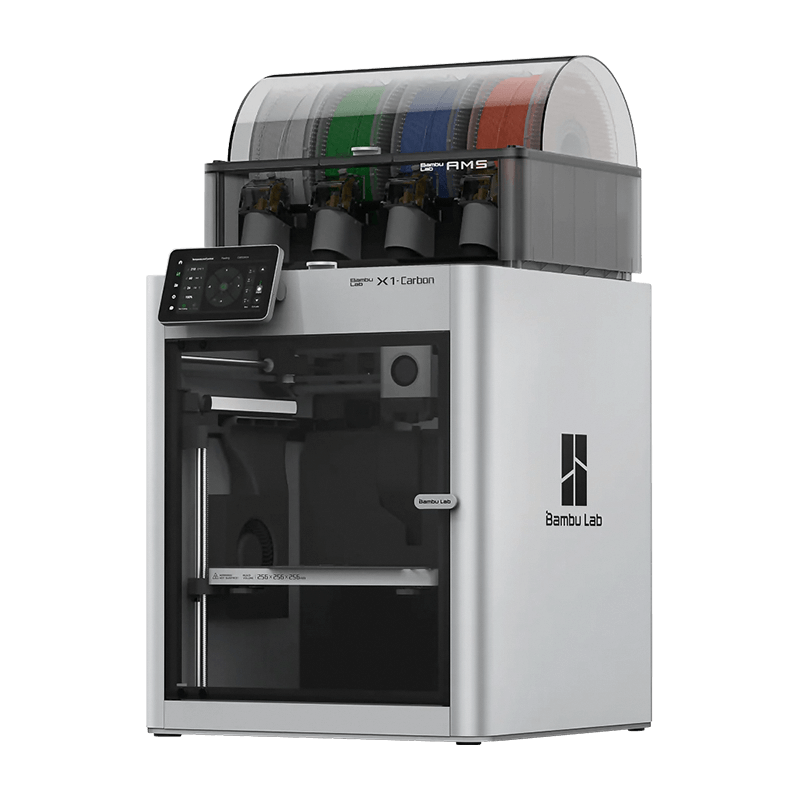
\includegraphics[width=0.8\linewidth]{images/3D-Drucker.png}
	\caption[Bambu Lab X1-Carbon 3 Pro]{Bambu Lab X1-Carbon 3 Pro}
	\label{fig:3D-Druck}
\end{figure}


\subsection{Vorteile des 3D-Drucks}
3D-Druck bietet viele Vorteile für Privatkunden und Unternehmen. Die nachfolgenden Vorteile zählen zu den wichtigsten:
\begin{itemize}
	\item Möglichkeit, komplexe Objekte relativ schnell herzustellen.
	\item Keine Vorlaufzeit nötig, d.h. keine Werkzeugproduktion erforderlich.
	\item Rapid Prototyping \emph{(deutsch „schnelle Prototypenherstellung“)}
	\item Kostengünstige Produktion
	\item Herstellung individueller Objekte
\end{itemize} \textcite{3DDruckVorteile}

\subsection{Nachteile des 3D-Druck}
3D-Druck bietet aber nicht nur Vorteile, sondern hat wie alle Technologien seine Nachteile und Schwächen.
\begin{itemize}
	\item Nachbearbeitung der Konstruktionen nötig.
	\item Nicht so genau wie subtraktive Fertigungverfahren.
	\item Lange Fertigungszeiten
	\item Begrenztes Bauvolumen
\end{itemize}
\textcite{3DDruckNachteile}

\subsection{Technische Voraussetzungen}
Um den 3D-Druck technisch durchführen zu können, werden folgende Komponenten benötigt:
\begin{itemize} 
	\item 3D-Drucker
	\item Slicer
	\item CAD-Programm
	\item 3D-Druck Material (Filament)
	\item Computer
\end{itemize}
Auf den nächsten Seiten wird auf diese Punkte näher eingegangen und ein Vergleich erstellt um die Vor- und Nachteile \textcite{3ds} der genannten 3D-Drucker zu veranschaulichen. 


\subsection{Druckverfahren}

Um Hardware mittels 3D-Drucks zu erstellen, gibt es verschiedene Möglichkeiten, das Ausgangsmaterial \textcite{3ds} in die gewünschte Form zu bringen. Die gängigsten und weitverbreitesten Verfahren \textcite{kaffka} im Überblick: 

\begin{itemize}
	\item \textbf{FFF:} (Fused Filament Fabrication) oder \textbf{FDM} (Fused Deposition Modelling): Hierbei wird Kunststofffilament \emph{(eine einzelne Faser beliebig lang)} verwendet und Schicht für Schicht aufgetragen.
	\item \textbf{SLA:} Diese Technologie verwendet lichtempfindliches Kunstharz, das sich verfestigt. Wird ebenfalls Schicht für Schicht aufgetragen.
	\item \textbf{PBF:} Eine Möglichkeit, diese pulverbasierte Technologie zu nutzen, ist, das Pulver mittels Laser miteinander zu verschmelzen.  
\end{itemize}
 

\subsection{Werkstoffe}
3D-Drucker benötigen zum Drucken eines Objektes Material, das sie verbrauchen können, um das Objekt herzustellen. Im Rahmen dieser Diplomarbeit werden zwei Werkstoffe ganuer analysiert, nämlich Nylon und Kohlefaser.

\subsubsection{Nylon}
Nylon \emph{(techn. Polyamid)} ist ein langlebiges Material, das sich vorallem durch seine Widerstandfähigkeit gegen Hitze und mechanischen Außeneinwirkungen auszeichnet \textcite{Nylon}. Nylon gibt es in unterschiedlichen Ausführungen zb. als Filament, Draht oder Pulver mit unterschiedlichen Eigenschaften. 
\subsubsection{Kohlefaser}
Kohlefasern wird in Grundpolymeren wie PLA oder Nylon eingearbeitet \textcite{Kohlefasern} um eine höhere Stabilität und Resistenz zu erzeugen wie zb. Nylon verstärkt mit Kohlefasern.\\
 


\subsection{3D-Drucker}

\subsubsection{Vergleich der 3D-Drucker}
Wie in der Einleitung des Kapitels \emph{"Hardware im Zusammenhang mit StageControl"} beschrieben, ist eine Möglichkeit zur Herstellung der benötigten Hardware das Drucken mittels eines 3D-Druckers. Um die bereits erwähnten 3D-Drucker (\emph{Bambu Lab X1-Carbon, Ultimaker 2 Extended+})  \textcite{Ultimaker2ExtendedSpecification} miteinander zu vergleichen, werden folgende Kriterien herangezogen: die Verarbeitbarkeit des Ausgangsmaterials und die Druckgeschwindigkeit bei einem Düsendurchmesser von 0,4 mm \textcite{BambuLabX1Carbon3DPrinterSpecifications}. 

Als Ausgangsmaterial wird bei beiden 3D-Druckern kohlefaserverstärktes Nylon-Filament verwendet.

\begin{table} [H]
	\begin{tabular}{ |p{2.7cm} |p{4.8cm}|p{4.8cm}| }
		\hline
		 \textbf{Kriterien} & \textbf{Ultimaker 2 Extended+}& \textbf{Bambu Lab X1-Carbon 3 Pro}\\
		\hline
		\textbf{Material} & Material kann verarbeitet werden & Material kann verarbeitet werden   \\ 
		\hline
		\textbf{Drucktempo} & Druckt mit einer Geschwindigkeit von 16mm\textsuperscript{3}/s &
		 Druckt mit einer Geschwindigkeit von 32mm\textsuperscript{3}/s   \\  
		\hline
		\textbf{Druckvolumen} & 223 x 223 x 205 mm & 256 x 256 x 256 mm \\
		\hline
		\textbf{Betriebssysteme} & MacOS, Windows, and Linux & Windows, MacOS \\
		\hline
	\end{tabular}
	\caption{Vergleich  Ultimaker 2 Extended+ und Bambu Lab X1-Carbon 3 Pro}
\end{table}


\subsection{Slicer}
\subsubsection{Was ist ein Slicer?}
Ein Slicer ist ein Stück Software, das es erst möglich macht 3D-Modelle auszudrucken, indem es einen sogenannten G-Code erstellt \textcite{SlicerGCode}. G-Code ist die Programmiersprache, die von Computern verwendet wird, um mit Maschinen zu kommunizieren, wenn die Maschine Bewegungen ausführen soll. \\



\section{CNC-Fräsen}

Ein weiterer Ansatz zur Hardware- bzw. Prototypenherstellung, der für StageControl benötigt wird, ist das CNC-Fräsen (\emph{engl. "Computerized Numerical Control"}). Diese Technologie wird vor allem in der metallverarbeitenden Industrie angewendet \textcite{CNCFraesen}, da sie äußerst genau und kostengünstig arbeitet. Zudem beschränkt sich das CNC-Fräsen nicht nur auf Metall; es kann auch bei der Bearbeitung von Kunststoffen und Holz eingesetzt werden \textcite{CNCFraesen2}. Anders als bei der 3D-Druck-Technologie handelt es sich hier nicht um ein additives, sondern um ein subtraktives Verfahren  \textcite{CNCFraesen3}..\\  


\begin{figure}[H]
	\centering
	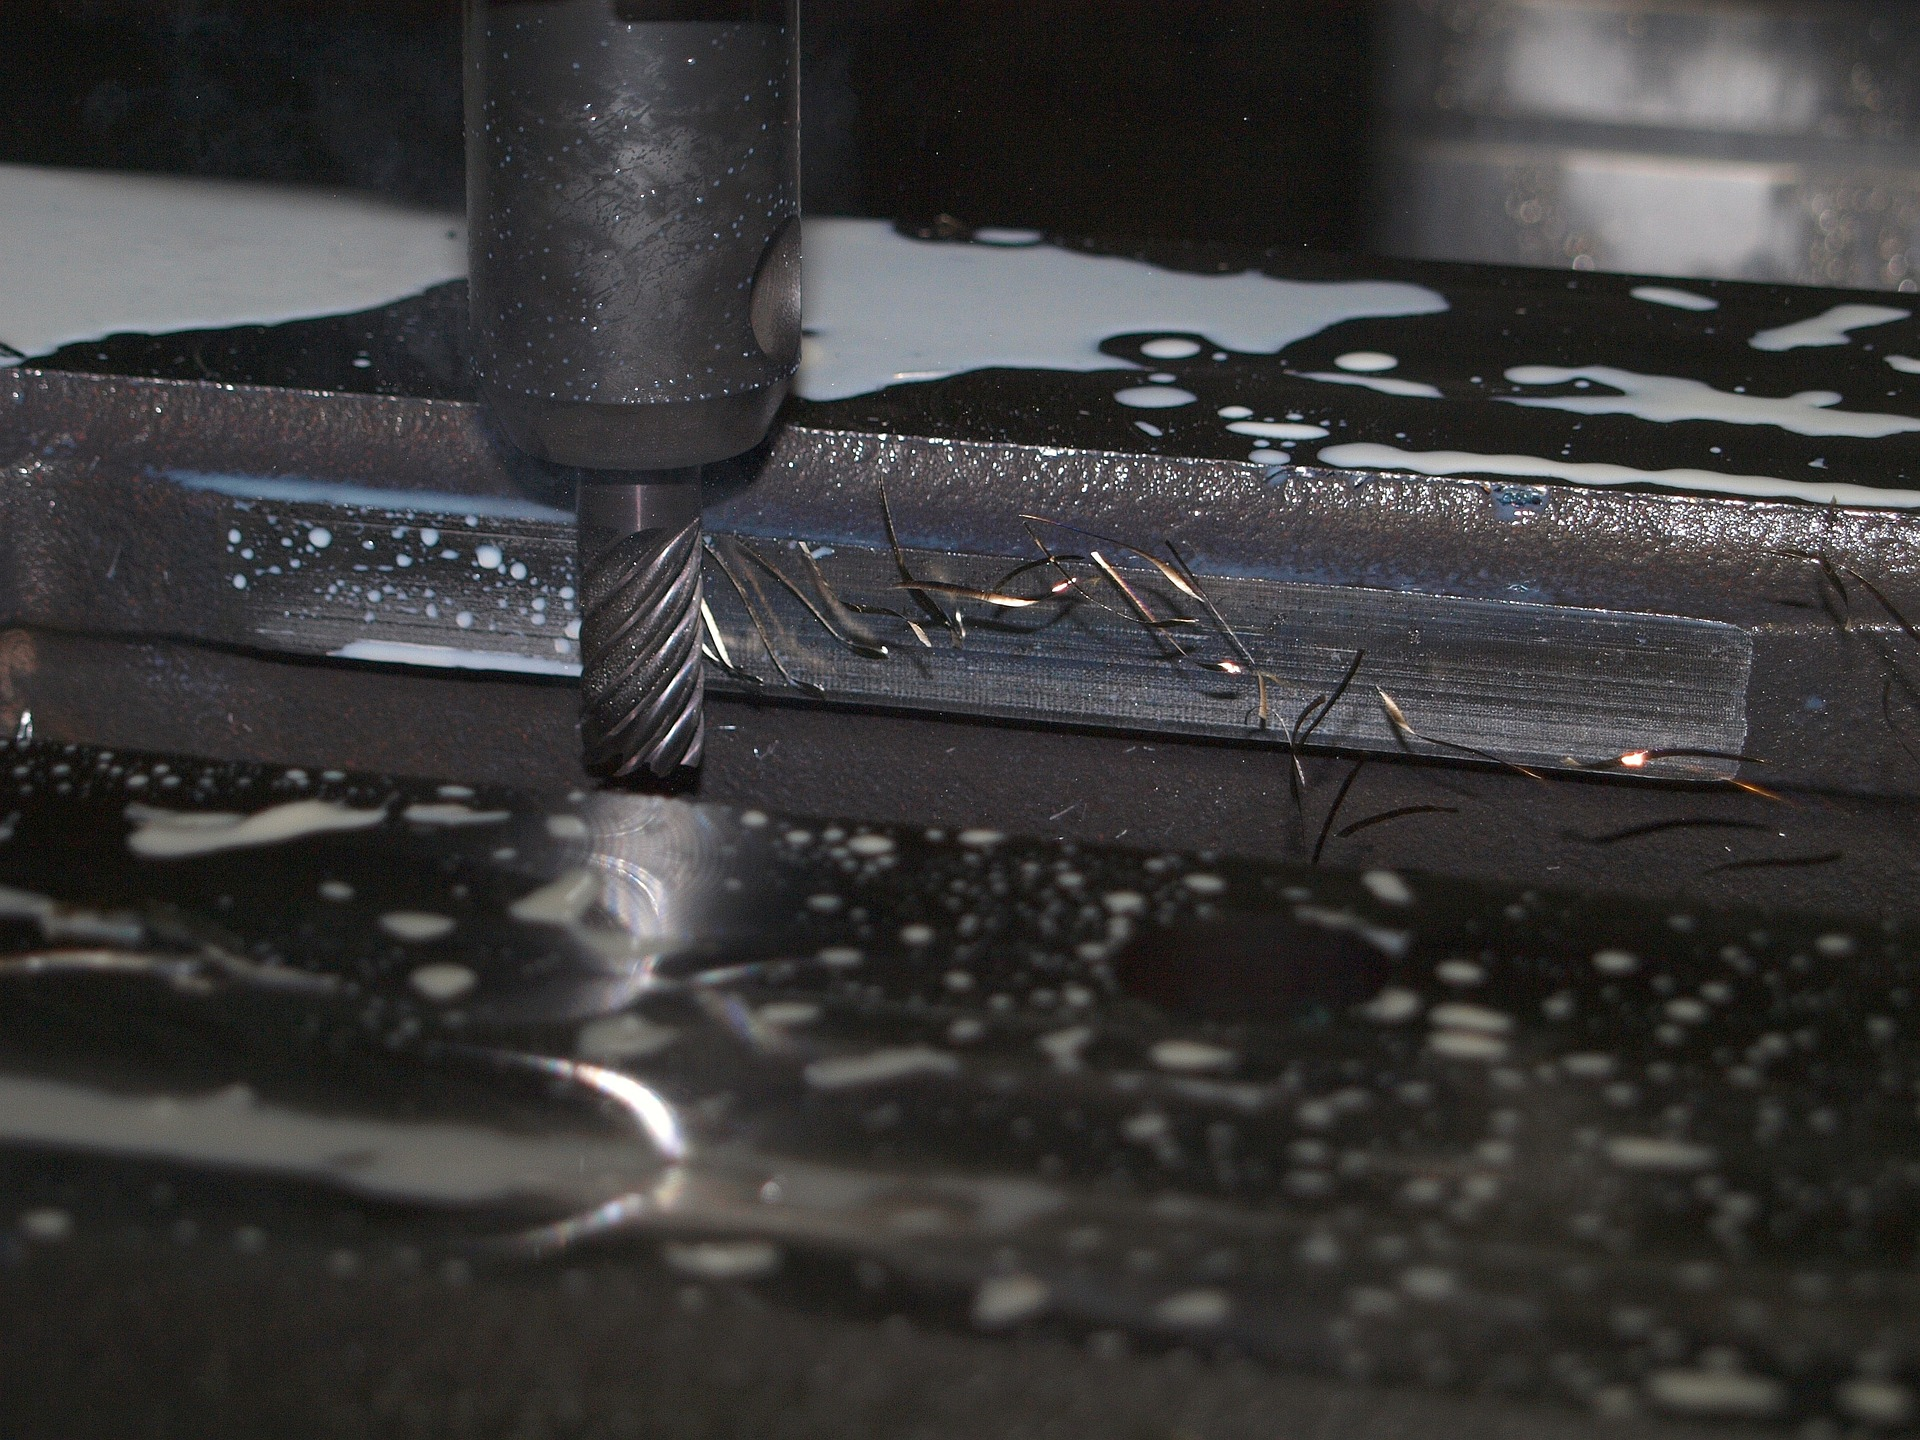
\includegraphics[width=0.8\linewidth]{images/CNC.jpg}
	\caption[CNC-Fräse]{CNC-Fräse}
	\label{fig:cnc-fraese}
\end{figure}

\subsection{Wie funktioniert CNC-Fräsen?}
Wie bereits in der Einleitung zum CNC-Fräsen erläutert, handelt es sich um ein subtraktives Verfahren, bei dem Material entfernt wird. Das Ausgangsmaterial wird fest in die Maschine eingespannt, während sich der Fräser bewegt \textcite{CNCFraesen2}. Der Fräser trägt dann das Material ab, um die gewünschte Form herzustellen. Um besonders präzise Abrundungen zu erzeugen, wird nicht das Material, sondern der Fräskopf fixiert, während sich das Material bewegt  \textcite{CNCFraesen3}. Wie beim 3D-Druck wird hier auch G-Code als Steuerung der Maschine eingestzt. \\



\subsubsection{Einsatzmöglichkeiten}
CNC-Fräsmaschinen können vielseitig eingesetzt werden und eine Vielzahl von Objekten in unterschiedlichsten Größen und Formen herstellen  \textcite{CNCFraesen2}. Zu den typischen Anwendungsbereichen zählen unter anderem:

\begin{itemize}
	\item Maschinenteilherstellung: Komponenten von Maschinen, die nur geringe Toleranzen zulassen.
	\item Prototypen: Herstellung von ersten Modellen in geringen Stückzahlen.
\end{itemize}

Durch den Einsatz von CNC-Fräsen können menschliche Fehler und die Ausschussrate minimiert werden. Dies führt zu niedrigeren Stückkosten, was sich besonders bei der Serienfertigung bemerkbar macht  \textcite{CNCFraesen3}..\\


\subsubsection{Vorteile des CNC-Fräsens}
CNC-Fräsen bietet im Vergleich zum herkömmlichen, manuellen Fräsen einige Vorteile. Wie bei jeder manuellen Arbeit können Arbeitsunfälle passieren. Durch den Einsatz moderner CNC-Fräsen, die aus der Ferne gesteuert werden können, lassen sich solche Unfälle reduzieren \textcite{CNCFraesenVorteile}. Ein weiterer Vorteil des CNC-Fräsens ist seine gleichbleibende Genauigkeit, da die CNC-Fräse computergesteuert ist. Diese Technologie wird vor allem bei Werkstücken eingesetzt, die nur wenig Toleranz in der Genauigkeit zulassen. CNC-Fräsen arbeiten mit einer Präzision von 0,01 bis 0,03 mm. \\


\subsection{CNC gesteuerte Maschinen}
Es gibt nicht nur CNC-Fräser oder Drehen, sondern alle Maschinen die durch CNC (\emph{engl. Computerized Numerical Control}) gesteuert werden, können als solche bezeichnet werden. Durch den Einsatz von CNC lassen sich die verschiedensten Maschinen computergestützt steuern. Zu diesen Maschinen zählen unter anderem CNC-Bohrmaschinen,  CNC-Laserschneidmaschinen, CNC-Schleifmaschinen, CNC-Wasserstrahlschneidmaschinen oder der 3D-Drucker \textcite{ArtenCNCMaschinen}
. \\


\subsection{Unterschied zwischen CNC-Fräsen und CNC-Drehen}
Beim CNC-Drehen wird ein Spannfutter anstatt des Schneidewerkzeugs eingesetzt. Dies ermöglicht die Herstellung von runden, zylindrischen oder konischen Formen. Mit diesem Verfahren lassen sich keine Objekte herstellen die eine hohe Präzision erfordern. Im Gegensatz zur CNC-Fräsmaschine arbeitet das CNC-Drehen nur auf zwei Achsen \textcite{CNCDrehenUnterschied}. Zudem dreht sich das Material und der Fräser ist fixiert, so wird das Material wie bei der CNC-Fräse abgetragen. \\



\subsection{Werkstoffe}
Bei der CNC-Fräsung können die unterschiedlichsten Materialien verwendet werden. Materialien, die eine CNC-Fräse verarbeiten kann, sind zerspanbar  \textcite{PEIZerspannung}. Zu den gängigsten zählen:

\begin{itemize}
	\item Metalle, z. B. Stahl, Aluminium, Titan, Bronze, Messing \textcite{CNCFraesen3}.
	\item Holz => Drechseln
	\item Zerspanbare Kunststoffe, z. B. PEI (\emph{Polyetherimid}), die sich durch ihre mechanische Festigkeit und Steifigkeit auszeichnen  \textcite{PEIKunststoffPolyetherimid}.
\end{itemize}


\subsection{Fertigungsmöglichkeiten}

\subsubsection{3-Achs-Fräsung}
Hierbei kann sich der Fräser auf drei Achsen bewegen, nämlich auf der X-, Y- und Z-Achse \textcite{Fraesen345Achs}. So kann das Material von allen drei Seiten bearbeitet werden. Es handelt sich um das einfachste Fräsverfahren. Zwar können auch komplexere Objekte erstellt werden, dies erfordert jedoch ein mehrfaches Umspannen des Werkstücks.

\subsubsection{4-Achs-Fräsung}
Zusätzlich zu den bereits bekannten drei Achsen kann nun eine vierte Achse integriert werden, nämlich das Schwenken der Aufspannung des Frästeils \textcite{Fraesen345Achs}. Dadurch kann das Umspannen, das bei der 3-Achs-Fräsung notwendig ist, vermieden werden.

\subsubsection{5-Achs-Fräsung}
Bei der 5-Achs-Fräsung kann nicht nur die Aufspannung des Frästeils zum Schwenken gebracht werden sondern auch der Maschinentisch selbst ist rotierbar. So kann das Werkstück von 5 Seiten in einer Aufspannung bearbeitet werden \textcite{Fraesen345Achs}. Diese Fräsen werden bei der Produktion höchstkomplexer Strukturen eingestzt.\\



\section{3D-Modellierungsprogramme}
Auf dem Markt rund um 3D-Modellierungsprogramme gibt es eine große Auswahl an den verschiedensten Programmen. Vom anfängerfreundlichen Tinkercad, das durch seine einfache Bedienbarkeit und zahlreiche Tutorials überzeugt, bis hin zu einem der führenden CAD-Programme wie Catia  \textcite{3DPrintingSoftware}, das in der Industrie für seine leistungsstarken und umfangreichen Funktionen geschätzt wird, ist alles dabei \textcite{CADProgramme},. Im Rahmen dieser Diplomarbeit wurden einige der Marktführer recherchiert und miteinander verglichen. \\


\subsection{Vergleich verschiedener Software}

\subsubsection{Autodesk Fusion}
Es eröffnet zahlreiche Anwendungsmöglichkeiten, die von der Prototypenerstellung bis hin zur Entwicklung von Konsumgütern reichen. Dieses Programm bietet umfangreiche Werkzeuge für Design, Engineering und Fertigung.  Fusion 360 wird von vielen internationalen und nationalen Unternehmen verwendet, weil es vielseitig einsetzbar ist und sowohl in kleinen als auch in großen Projekten hervorragende Unterstützung bietet \textcite{AutodeskFusion}. Dank seiner cloudbasierten Plattform ermöglicht Fusion 360 eine nahtlose Zusammenarbeit und den einfachen Austausch von Projektdaten, was es zu einer bevorzugten Wahl in der modernen Produktentwicklung macht. \\


\textbf{Vorteile}
\begin{itemize}
	\item Genutzt von vielen namhaften Unternehmen wie zb. Yamaha oder Panasonic
	\item Große Community
	\item Kostenlose Version für Schulen \textcite{AutodeskFusionReviews}
\end{itemize} 

\textbf{Nachteile}
\begin{itemize}
	\item Cloud Based; Kann zu Problemen führen, wenn offline genutzt 
	\item Benötigt eine schnelle Internetverbindung
	\item Hoher Anspruch an die Hardware des Computers \textcite{AutodeskFusionReviews}
\end{itemize}



\subsubsection{Blender} 
Blender bietet vielseitige Anwendungsmöglichkeiten, von Modellierung und Animation bis hin zur Spieleentwicklung und visuellen Effekten. Dieses Open-Source-Programm bietet umfassende Werkzeuge für Modellierung, Simulation, Rendering, Compositing und Motion Tracking. Zudem wird Blender von vielen internationalen und nationalen Unternehmen sowie unabhängigen Kunden bzw. Kundinnen verwendet, weil es viele Einsatzmöglichkeiten bietet und gratis zugänglich ist \textcite{Blender}. Dank seiner aktiven Community und regelmäßigen Updates bleibt Blender immer auf dem neuesten Stand der Technik. \\


\textbf{Vorteile}
\begin{itemize}
	\item Gratis 
	\item Open Source Software
	\item Funktioniert auf allen gängigen Betriebssystemen
	\item Regelmäßige Updates
	\item große Community \textcite{BlenderProsUndCons}
\end{itemize}

\textbf{Nachteile}
\begin{itemize}
	\item Kein Industriestandard - wird nicht von großen Unternehmen genutzt
	\item Nicht die benutzerfreundlichste Oberfläche \textcite{BlenderProsUndCons}
\end{itemize}



\subsubsection{FreeCAD}
FreeCAD hat vielseitige Anwendungsmöglichkeiten, von der Modellierung bis hin zur Erstellung technischer Zeichnungen und Simulationen. Diese Open-Source-Software bietet umfassende Werkzeuge für Ingenieure, Architekten, Produktdesigner und Privatkunden \textcite{FreeCAD}. Zudem wird FreeCAD von vielen Unternehmen sowie unabhängigen Entwicklern und Entwicklerinnen genutzt, weil es flexible Einsatzmöglichkeiten bietet. Durch seine modulare Architektur und der aktiven Community wird FreeCAD kontinuierlich weiterentwickelt und verbessert   \textcite{FreeCAD2}. \\


\textbf{Vorteile}
\begin{itemize}
	\item Open Source Software
	\item Gratis
	\item Funktionsfähig für alle gängigen Betriebssysteme
	\item Aktive Community \textcite{FreeCADReviews}
\end{itemize}

\textbf{Nachteile}
\begin{itemize}
	\item weniger Nutzer und Nutzerinnen als die bereits genannten Programme
	\item kein Industriestandard
	\item limitierte Funktionalitäten im Vergleich zu Bezahlsoftware \textcite{FreeCADReviews}
\end{itemize}

\subsubsection{Autodesk Tinkercad}
Autodesk Tinkercad ist ein für Anfänger und Anfängerinnen und Schüler und Schülerinnen entwickeltes Online-Tool. Wie der Name es schon verrät, ist es ein Produkt von Autodesk, wie das vorher genannte Autodesk Fusion 360. Dieses webbasierte Programm erfüllt alle grundlegenden Anforderungen und bietet intuitive Werkzeuge für Schüler und Schülerinnen, Lehrer und Lehrerinnen und Privatpersonen. Zudem wird Tinkercad von vielen Bildungseinrichtungen verwendet, weil es leicht zugänglich und einfach zu erlernen ist \textcite{Tinkercad}. Dank seiner klaren Benutzeroberfläche und umfangreichen Tutorials ermöglicht Tinkercad einen schnellen Einstieg in die Welt des 3D-Designs und der Elektronik. \\


\textbf{Vorteile}
\begin{itemize}
	\item Gratis
	\item Benutzerfreundliches UserInterface (\emph{Nutzeroberfläche})
	\item intuitives Design
	\item Online Tool - kein Download 	
	\item viele einsteigerfreundliche Tutorials \textcite{TinkercadReviews}
\end{itemize}

\textbf{Nachteile}
\begin{itemize}
	\item Weniger professionell
	\item kein Industriestandard \textcite{TinkercadReviews}
\end{itemize}

\section{Mischpult}
 Für StageControl benötigen wir zur Ansteuerung einer Tonanlage ein Mischpult, um den von uns gewünschten Stereoeffekt zu erzeugen. Mischpulte, auch Mixer genannt, gibt es in ganz unterschiedlichen Größen. Die Größe hängt meist von der Anzahl der Kanäle ab, die das Mischpult bietet. Mischpulte werden immer dann verwendet, wenn mehrere Audiosignale verarbeitet werden müssen, wie auf Bühnen oder in Proberäumen \textcite{MischpultInformation}. Bei allen Mischpulten gibt es eine sogenannte Leserichtung, die den Aufbau des Mischpults beschreibt. Von links nach rechts findet man die einzelnen Kanäle, und von oben nach unten die Bearbeitungsmöglichkeiten des Tons. Dazu kommt noch der sogannte Masterbereich. Hier wird alles gesteuert, was zentral gereglt werden muss. Diese Einstellungen gelten dann für alle Kanäle  \textcite{MischpultMaster}. \\
 

\begin{figure}[H]
	\centering
	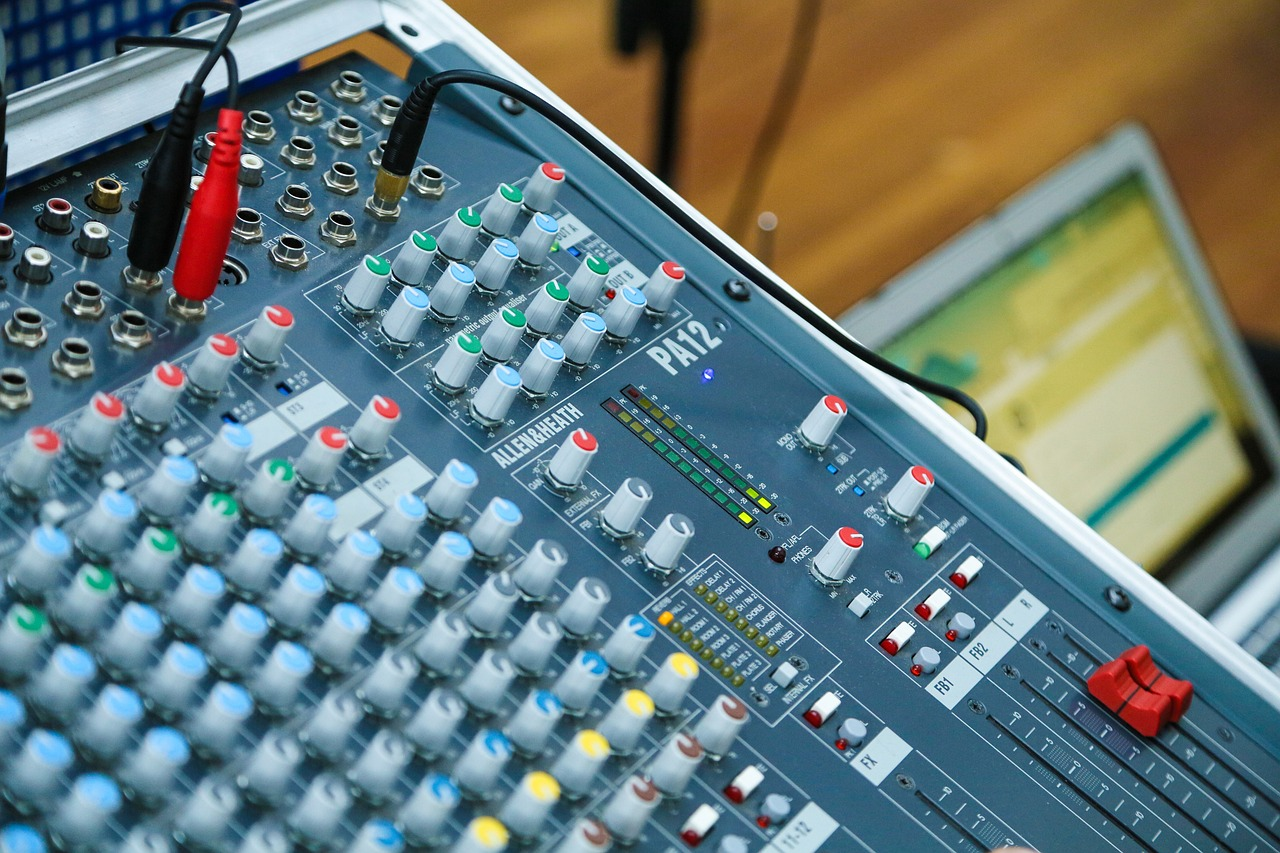
\includegraphics[width=0.8\linewidth]{images/mischpult.jpg}
	\caption[Mischpult]{Mischpult}
	\label{fig:Mischpult}
\end{figure}

\subsection{Funktionsweise eines Mischpults}
Im Grunde summiert ein Mischpult alle Tonquellen zu einen einzigen Signal. So kann dann dieses Signal über die Tonanlage ausgegeben werden \textcite{MischpultErklaerung}. Bei Mischpulten gibt es eine Vielzahl von Knöpfen und Reglern für jeden Kanal, diese sind wie schon erwähnt zur Bearbeitung des Tones da, im Rahmen dieser Diplomarbeit wird auf dies nicht genauer eingagangen. \\


\subsection{Einsatzmöglichkeiten}
Mischpulte finden eine Vielzahl von Anwendungsmöglichkeiten, wie z.B. auf Bühnen oder in Proberäumen. Mischpulte übernehmen eine Bandbreite von Aufgaben \textcite{MischpultVerwendungszweck}. Die folgenden gehören zu den Wichtigsten:
\begin{itemize}
	\item Signalverstärkung
	\item Bearbeitung von Signalen
	\item Signale zum Aufnahmesystem schicken
\end{itemize}


\subsection{Unterschied Digital/Analog}
\subsubsection{Digital}
Unter einem digitalen Mischpult versteht man ein Mischpult, das analoge Signale in digitale Signale umwandelt und diese Signale mittels Software bearbeitet. Um ein digitales Signal wieder über eine Tonanlage auszugeben, muss es erneut in ein analoges Signal umgewandelt werden. Dies führt wiederum zu Latenzzeiten bei der Signalausgabe.
\subsubsection{Analog}
Im Gegensatz dazu steht das analoge Mischpult. Es wandelt die Signale nicht in digitale um, sondern behält deren ursprüngliche analoge Form bei und bearbeitet sie ohne Software weiter \textcite{MischpultAnalogDigital}. Ohne diese Umwandlung gibt es nahezu keine Latenzzeit bei der Ausgabe der Signale. \\


\subsection{Anforderungen für StageControl}
Für StageControl ist es besonders wichtig, dass das verwendete Mischpult entweder jeden Kanal einzeln panen (\emph{Regler zu Ausrichtung des Tons (links/Rechts)}) kann oder das der Master mindestens zwei Lautsprecher einer Tonanlage einzeln ansteuern kann. Somit kann der von uns gewünschte Stereoeffekt erzeugt werden. \\
Für StageControl wird ein Mischpult mit Drehreglern verwendet, da diese häufig in kostengünstigeren Mischpulten zu finden sind und für die Anforderungen dieser Arbeit vollkommen ausreichen. 



\subsection{Vergleich zweier Modelle}
Wie am Anfang des Kapitels \emph{Mischpult} beschrieben benötigt StageControl ein Mischpult, um den von uns gewünschten Stereoeffekt zu erzeugen. Hierzu werden zwei Mischpulte herangezogen \textcite{MischpultKriterien1204}, die unseren Kriterien entsprechen und  verglichen  \textcite{MischpultKriterien1402}.

\begin{table} [H]
	\begin{tabular}{ |p{3.1cm} |p{4.8cm}|p{4.8cm}| }
		\hline
		\textbf{Kriterien} & \textbf{Behringer Xenyx 1204USB}& \textbf{the t.mix xmix 1402 USB}\\
		\hline
		\textbf{Kosten} & 169€ & 168€  \\ 
		\hline
		\textbf{Digital/Analog} & Analog & Analog   \\  
		\hline
		\textbf{Master kann zwei Lautsprecher seperat ansprechen} & Ja & Ja \\
		\hline
		\textbf{PC-Schnittstelle} & USB-B & USB-B  \\
		\hline
		\textbf{Gewicht}& 2.8 kg & 4.8 kg \\
		\hline	
	\end{tabular}
	\caption{Vergleich Behringer Xenyx 1204USB und the t.mix xmix 1402 USB} 
\end{table} 

\section{Lichtsteuerung}
Ein weiterer Aspekt dieser Diplomarbeit ist die gleichzeitige Ansteuerung von Ton- und Lichtanlagen, wie z.B. einem Spotlight (\emph{deutsch Verfolgungsscheinwerfer}), das den Künstler bzw. der Künstlerin auf der Bühne verfolgt. Auf Bühnen wird nicht nur ein Spotlight eingesetzt, sondern ganze Anlagen von Lichtern. Dies wird gemacht, um für den Zuschauer eine immersive Vorstellung zu bieten. 

\begin{figure}[H]
	\centering
	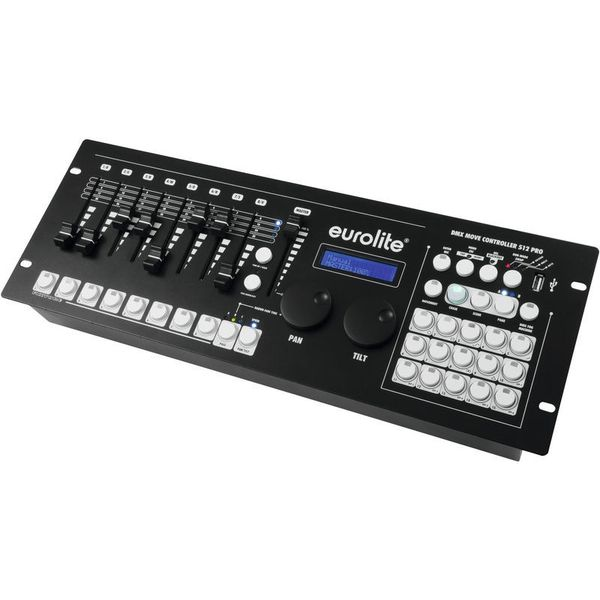
\includegraphics[width=0.7\linewidth]{images/DMX_Controller.jpg}
	\caption[DMX Controller]{DMX Controller}
	\label{fig:DMX_Controller}
\end{figure}

\subsection{Lichtanlagen bei StageControl}
Im Fall von StageControl wird keine vollständige Lichtanlage verwendet; es kommt lediglich ein Scheinwerfer zum Einsatz, um die Beleuchtung des Künstlers bzw. der Künstlerin via Positionsverfolgung zu ermöglichen. So erhalten wir die genaue Abstimmung von Ton und Licht auf die Person.

\subsection{Ansteuerung von Lichtanlagen}

Die gängigsten Arten der Ansteuerung von Lichtanlagen sind das DMX-Protokoll (\emph{Digital Multiplex}) oder das RDM-Protokoll (\emph{Remote Device Management}). Zur Ansteuerung der Lichtanlagen selbst wird ein DMX-Controller benötigt, der die Scheinwerfer steuert. Es wird ein DMX-Controller mit einem DMX-Ausgang und ein Scheinwerfer mit einem DMX-Eingang gebraucht.
\textbf{DMX} ist das am häufigsten verwendete Protokoll zur Lichtansteuerung in der Bühnentechnik. Moving-Heads, Lichteffekte und viele mehr werden in der Regel mithilfe von Lichtsteuerpulten über das DMX-Protokoll angesteuert und/oder programmiert \textcite{LichtanlageRDMDMX}.
\textbf{RDM} basiert auf dem DMX-Protokoll, erlaubt aber im Halbduplexbetrieb Rückmeldungen, was das Einrichten deutlich erleichtern kann.\\


\subsection{Hartes bzw. weiches Licht}
Es gibt zwei Lichtarten, die man in der Lichttechnik unterscheiden kann, nämlich hartes und weiches Licht. Beide Arten bieten sich für unterschiedliche Einsatzmöglichkeiten an. Weiches Licht wird meist eingesetzt, um größere Bereiche auszuleuchten. Auf der anderen Seite der Lichtskala gibt es das harte Licht, das sehr präzise eingesetzt werden kann, wie im Fall von StageControl bei der Verfolgung des Künstlers/der Künstlerin auf einer Bühne. Bei Scheinwerfern, die hartes Licht ausstrahlen, kommt das Licht von einem Punkt aus \textcite{HartesWeichesLicht}. Hingegen wird weiches Licht von einer Fläche aus abgestrahlt.\\


\subsection{Arten von Scheinwerfern}
In der Lichttechnik gibt es verschiedenste Scheinwerfertypen, die unterschiedliche Aufgaben besonders gut erfüllen. Zwei Scheinwerfertypen, die im Rahmen dieser Diplomarbeit zum Einsatz kommen, werden genauer erklärt.

\subsubsection{Verfolgerscheinwerfer}
Der Verfolgerscheinwerfer wird verwendet, um Personen auf Bühnen zu verfolgen. Diese Scheinwerfer werden nicht wie andere Scheinwerfer fix montiert, sondern lassen sich bewegen, um den gewünschten Verfolgungseffekt zu bieten. Dies geschieht nicht automatisch, sondern wird manuell von einem Beleuchter während der Show durchgeführt \textcite{Verfolgerscheinwerfer}. Es gibt verschiedene Lösungsansätze zur Bewegung von Movinglights (\emph{deutsch „Bewegbare Lichter“}). \ Bei Konzerten wird ein Verfolgerscheinwerfer oberhalb der Bühne gemeinsam mit dem Beleuchter platziert. Dieser steuert dann das Licht über ein Bedienfeld während der Performance.\\


\begin{figure}[H]
	\centering
	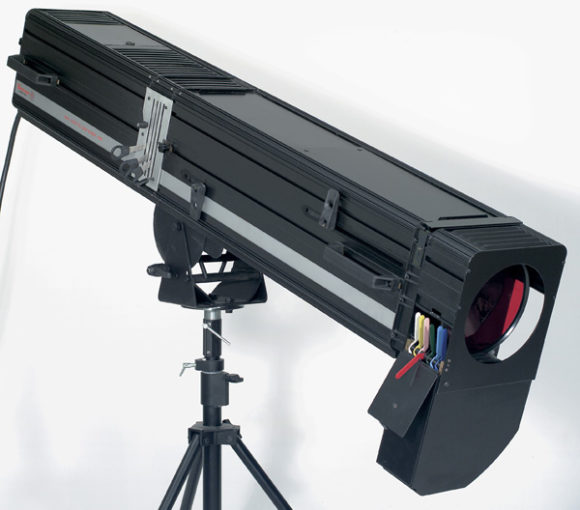
\includegraphics[width=0.7\linewidth]{images/Verfolgerscheinwerfer.jpg}
	\caption[Verfolgerscheinwerfer]{Verfolgerscheinwerfer}
	\label{fig:Verfolgerscheinwerfer}
\end{figure}

\subsubsection{Profilscheinwerfer}
Dieser Scheinwerfertyp wird vor allem im Theaterbereich eingesetzt. Ein enormer Vorteil des Profilscheinwerfers ist, dass er ein hartes und exaktes Licht ausstrahlt. Außerdem ist das Streulichtaufkommen deutlich geringer als bei anderen Scheinwerfern. Streulicht ist das Licht, das außerhalb des eigenlichen Lichtkegels auftritt. Zudem verfügen Profilscheinwerfer über einen Zoom, der manuell oder automatisch erfolgen kann \textcite{Profilscheinwerfer}. Dieser Scheinwerfertyp bietet zusätlich eine Scharfstellfunktion/Fokus mittels Linsenverschiebung an, diese wird durch den Linsentubus ermöglicht.\\


\begin{figure}[H]
	\centering
	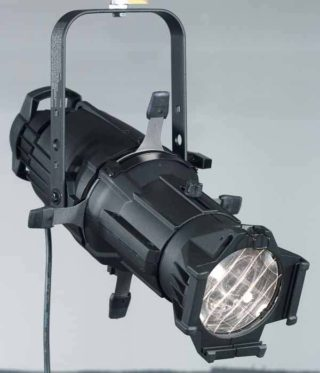
\includegraphics[width=0.7\linewidth]{images/Profilscheinwerfer.jpg}
	\caption[Profilscheinwerfer]{Profilscheinwerfer}
	\label{fig:Profilscheinwerfer}
\end{figure}

\section{Servomotoren}
\subsection{Einsatz von Servos bei StageCotrol}
Servomotoren werden für die Umwandlung der physischen Bewegung des Künstlers, in mechanische Bewegung des Servomotors benötigt, um so die Regler des Mischpults in Abstimmung und Ausrichtung des Künstlers mit dem Ton zu automatisieren. Diese Servomotoren werden oberhalb des Mischpult mithilfe des Gerüsts plaziert, wie in Kapitel 2.2.1 beschrieben. Diese Motoren sind essenziell für den Erfolg, da ohne diese Servos keine Automatisierung erfolgen kann.

\subsection{Was ist ein Servomotor}
Unter einem Servomotor wird keine Bauart eines Motors verstanden, sondern vielmehr spezielle Eigenschaften. Diese Eigenschaften sind: Strom-, Drehzahl- und/oder Positionsgeregelt. Ein Servomotor ist immer elektrisch betrieben. Diese Motoren geben Rückmeldungen an die Regelelektronik. Diese Rückmeldungen enthalten Informationen über Winkelposition der Motorwelle, der Drehgeschwindigkeit und der Beschleunigung \textcite{ServomotorInfo}. Die Regelelektronik kann anhand dieser zurückgemeldeten Daten wieder die Daten der Sollparameter an den Motor schicken, die zuvor eingegeben wurden. \\


\subsection{Anforderungen für StageControl}
Für den Einsatz bei StageControl gibt es Vorraussetzungen, die die Servomotoren erfüllen müssen, ehe sie in Erwägung gezogen werden. Diese Kriterien sind: Drehung des Motors im und gegen den Uhrzeigersinn, Kompaktheit, passenende Schnittstelle (Bus/Analog/Digital) für die Eingabe der Sollzustände und die Rückmeldung der Aktuellen Position.

\begin{figure}[H]
	\centering
	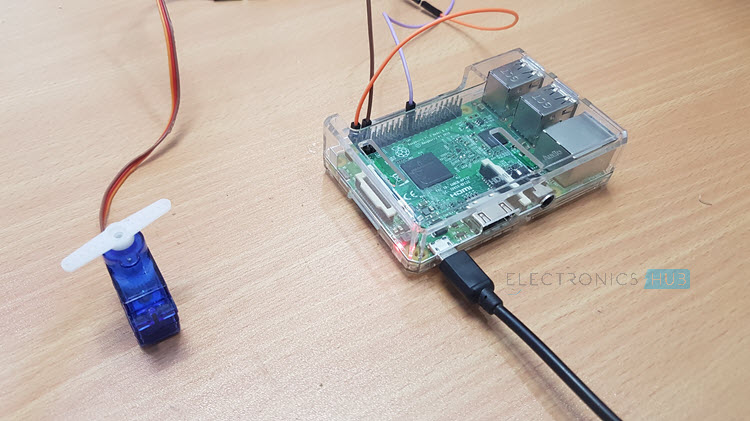
\includegraphics[width=0.7\linewidth]{images/servo.jpg}
	\caption[Servomotor]{Servomotor}
	\label{fig:Servo}
\end{figure}

\subsection{Arten von Servomotoren}
Es gibt einige unterschiedliche Arten von Servos, die wichtigsten drei sind: Gleichstrom, kernlose und bürstenlose Motoren. \\
Bei Gleichstromservos handelt sich um die billigste und gängiste Art der Motoren. Dieser Servotyp besteht aus Eisenkernen um die Kupferdraht gewickelt ist, sowie einem Kommutator Ring und Bürsten. Diese Bürsten werden zur Umschaltung der Felder benötigt und einem Gehäuse. \\
Kernlose Motoren sind erheblich teuerer in der Produktion als Gleichstrommotoren, da diese aus teurern Materialien bestehen. Ihr großer Vorteil gegenüber herkörmlicher Gleichstrommotoren ist, das diese deutlich schneller beschleunigen und abbremsen können \textcite{ServomotorArten}. \\
Anstelle der Bürsten und dem Metallring bei Bürstenservos, wird bei den Bürstenlosen Servos Elektronik, die den Motor steuert, eingebaut um die selbe Zuverlässigkeit zu gewährleisten. Der Einbau von Elektronik zeichnet sich durch die längere Lebensdauer des Servos aus. Durch die Elektronik fallen diese Motoren deutlich teurer aus als Gleichstrommotoren. \\



\subsection{Ansteuerung von Servos}
Servomotoren werden über ein sogenanntes PWM-Signal (\emph{Pulsweitenmodulations-Signal}) gesteuert. Dies bedeutet, dass der Servomotor über elektrische Pulse angesteuert wird und so die Befehle erhält, auf welche Postion er fahren muss. Diese Motoren werden üblicherweise über drei Kabeln mit dem Steuerunggerät verbunden. Das erste Kabel ist das Massekabel, dies ist für die Rückleitung der Pulse verantwortlich. Nummer zwei ist das Versorgungsspannungskabel, dies versorgt den Servomotor mit der nötigen elektrischen Spannung \textcite{ServomotorAnsteuerung}. Das dritte Kabel ist das Signalleitungskabel, dieses Kabel leitet die Pulse an den Servo weiter, so wird dem Servo die anzufahrende Position mitgeteilt.\\


\begin{figure}[H]
	\centering
	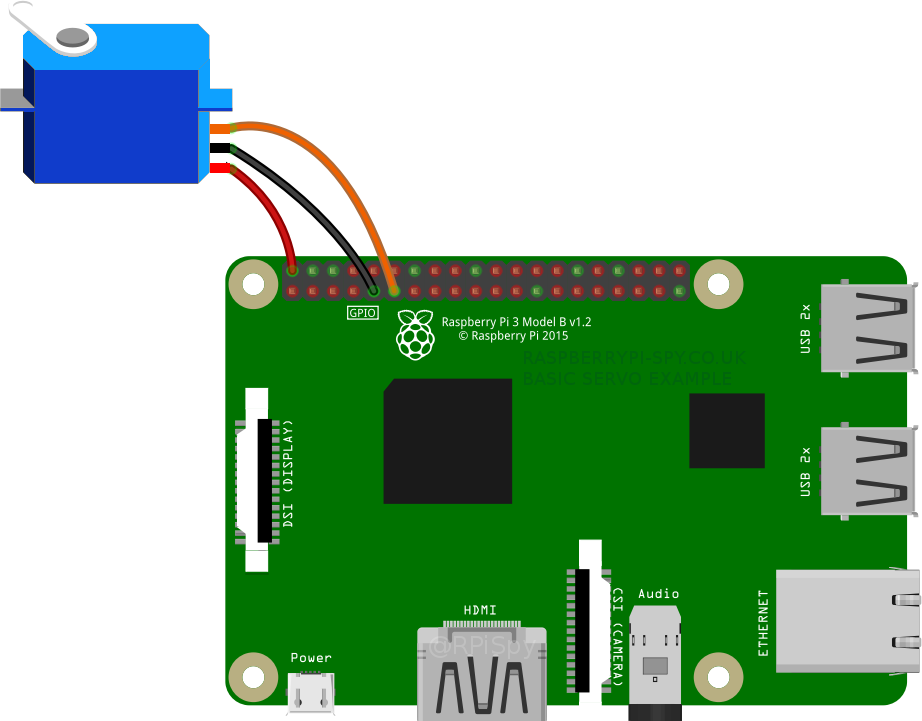
\includegraphics[width=0.7\linewidth]{images/Pin_Belegung.png}
	\caption[Pin-Belegung Servo]{Pin-Belegung Servo}
	\label{fig:PIN_Belegung}
\end{figure}

\section{Navigation}

Um die Licht- und Audioanlagentechnik richtig zu koordinieren benötigt man eine Art von Navigation. Da es sich meist um Bühnen im Innenbereich handelt, kann man keine übliche Technologie verwenden.


\subsection{GPS}
GPS (\emph{=engl. Global Positioning System}) \textcite{GPS} wird für die Standortermittlung im Außenbereich verwendet und ist für unseren Fall nicht verwendbar. Für die genaue Bestimmung von Positionen werden Satelliten verwendet.

\textbf{Funktionsweise des GPS}

Es gibt GPS-Satelliten die, die Erde zweimal pro Tag umkreisen in einer genauen Umlaufbahn. Diese Satelliten senden eindeutige Signale und Bahnparameter aus, somit können die genauen Postionen der GPS-Geräte bestimmt werden. 
In so gut wie jeden neuen Geräten ist das GPS-standart und werden für die verschiedensten Funktionen verwendet. Durch die Positionsermittlung können folgende andere Informationen berechnet werden:

\begin{itemize}
	\item Geschwindigkeit
	\item Peilung
	\item Track
	\item Reisedistanz
	\item Distanz zum Ziel
	\item Zeiten von Sonnenaufgang und Sonnenuntergang
\end{itemize}

\textbf{Signal}

Wenn GPS-Signale die Erde erreichen, sind die gesendeten Signale sehr schwach. Deshalb kommt es auch zu Problemen beim Durchdringen von Objekten wie Gebäuden o. Ä. Bei modernen GPS-Empfängern ist eine Indoor-Ortung möglich.

\textbf{Fehlerquellen für die Genauigkeit der GPS-Signale}

Es gibt einige relevante Fehlerquellen für GPS-Signale darunter fallen \textcite{GPSFehlerquellen}:
\begin{itemize}
	\item Position der Satelliten
	\item Signaleffekt der Umgebung
\end{itemize}


\textbf{Position der Satelliten}

Um ein Objekt zu positionieren sind mindestens drei Satelliten notwendig und einen weiteren, um etwägige Fehler zu beseitigen. Grundsätzlich gilt: Desto mehr Satelliten, desto genauer die GPS-Genauigkeit. Außerdem sollte das Signal von gleichmäßig verteilten Satelliten kommen, ist die GPS-Genauigkeit höher. Für die Berechnung dieser Genauigkeit gibt es den Dilution of Precision (= DOP) Wert.  Je kleiner dieser Wert, desto genauer ist das GPS-Signal.
\begin{figure}[H]
	\centering
	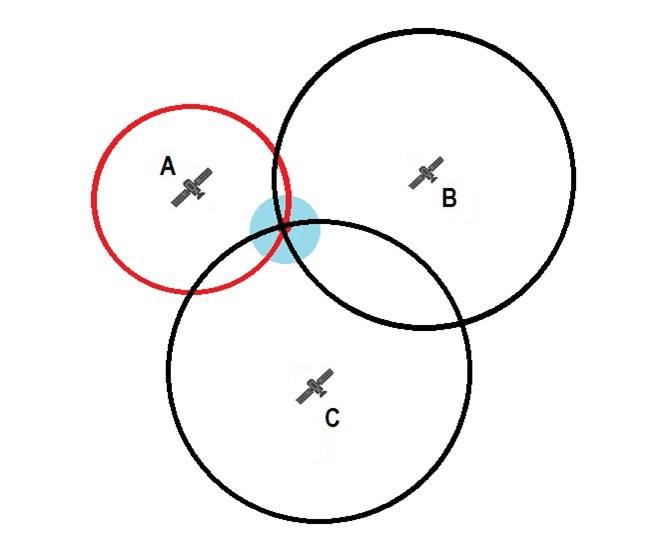
\includegraphics[width=0.7\linewidth]{images/Satellitenposition.jpg}
	\caption[Satellitenpositionierung]{Satellitenpositionierung}
	\label{fig:Satellitenposition}
\end{figure}

\textbf{Signaleffekt der Umgebung}


Bis die Signale von Satelliten schlussendlich beim GPS-Empfänger ankommen legen sie eine lange Stecke zurück, die Ausbreitungsumgebung beinflusst nicht nur die Siganlestärke, sondern auch die Genauigkeit, stark.
\begin{figure}[H]
	\centering
	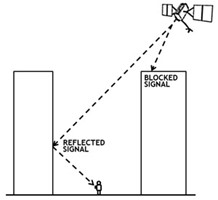
\includegraphics[width=0.7\linewidth]{images/Satelliteneinfluss.jpg}
	\caption[Satelliteneinfluss]{Satelliteneinfluss}
	\label{fig:Satelliteneinfluss}
\end{figure}

\subsection{ESP32}

ESP32 ist eine Reihe von Chip-Mikrocontrollern, die von dem Unternehmen Espressif entwickelt wurden und mit Hilfe von Arduino bzw. der Programmiersprache C kommunizieren. Der ESP32 \textcite{ESP32} zeichnet sich mit folgenden Dingen aus:

\begin{itemize}
	\item niedrige Anschaffungskosten
	\item geringer Stromverbrauch
	\item Wi-Fi
	\item Bluetooth
\end{itemize}


\begin{figure}[H]
	\centering
	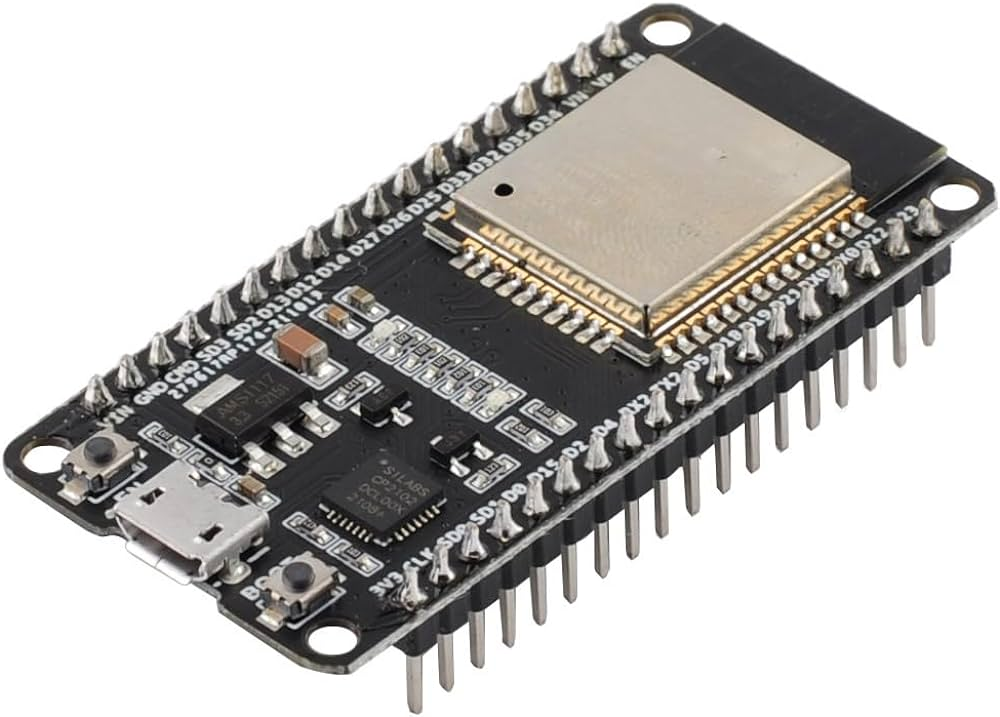
\includegraphics[width=0.7\linewidth]{images/ESP32.jpg}
	\caption[ESP32]{ESP32}
	\label{fig:ESP32}
\end{figure}

\textbf{Anschaffungskosten \& Stromverbrauch}

Der Mikrocontroller ist bereits ab einem Preis von \$6 erhältlich. Außerdem verbraucht dieser im Vergleich zu anderen Mikrocontrollern sehr wenig Strom und unterstützt Energiesparmodule, wie Tiefschlaf.

\textbf{Funktionen}

Der Mikrocontroller bietet nicht nur Wi-Fi (\emph{=Wireless Local Area Network}), sondern auch Bluetooth. Mit der Wireless Local Area Network Funktionen kann man einfach und drahtlos eine Verbindung zu einem Netzwerk herstellen und somit eine Kommunikation von vielen Geräten möglich machen. Außerdem verfügt der Mikrocontroller über Bluetooth-Classic.

\subsection{ESP32-Spezifikationen}

\begin{itemize}
	\item Bluetooth Classic und Bluetooth Low Energy
	\item Tensilica Xtensa Dual-Core 32-Bit LX6 Mikroprozessor, 160 oder 240 MHz
	\item ROM:  448 KB
	\item SRAM:  520 KB 
\end{itemize}

\subsection{MPU-6050}

Für weitere Funktionen benötigt man z.B. die Erweiterungsplatine MPU-6050, diese bringt einen Beschleunigungssensor und ein Gyroskop mit. Diese Platine beläuft sich auf einen Preis von ca. \$3.

\begin{figure}[H]
	\centering
	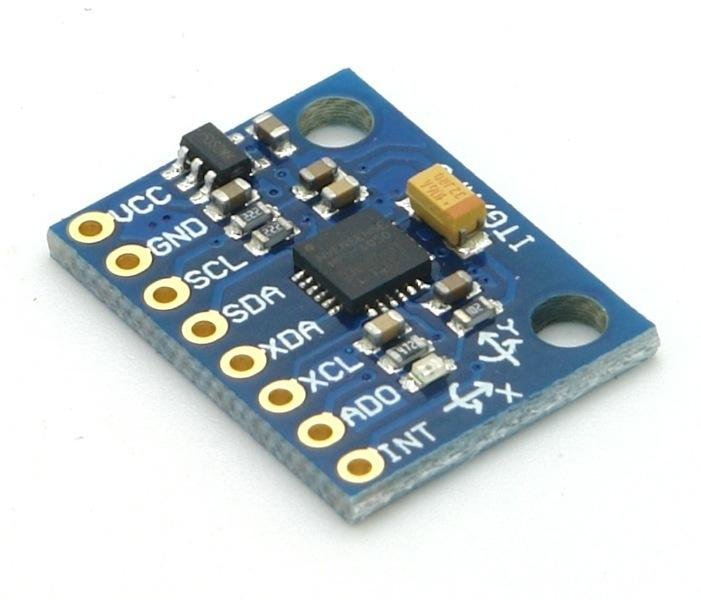
\includegraphics[width=0.7\linewidth]{images/MPU6050.jpg}
	\caption[MPU6050]{MPU-6050}
	\label{fig:MPU6050}
\end{figure}


\textbf{Gyroskop}

Jeder kennt die Wirkung eines Kreisel, ein Gyroskop hat genau diese und wird deshalb auch Kreiselinstrument genannt. Man nutzt die Wirkung, um die Lage eines Objektes zu bestimmen. Im Falle von einem MPU-6050 wird ein Sensor namens Micro-Electric-Mechanical Systems (\emph{kurz MEMS}) verwendet. 


\begin{figure}[H]
	\centering
	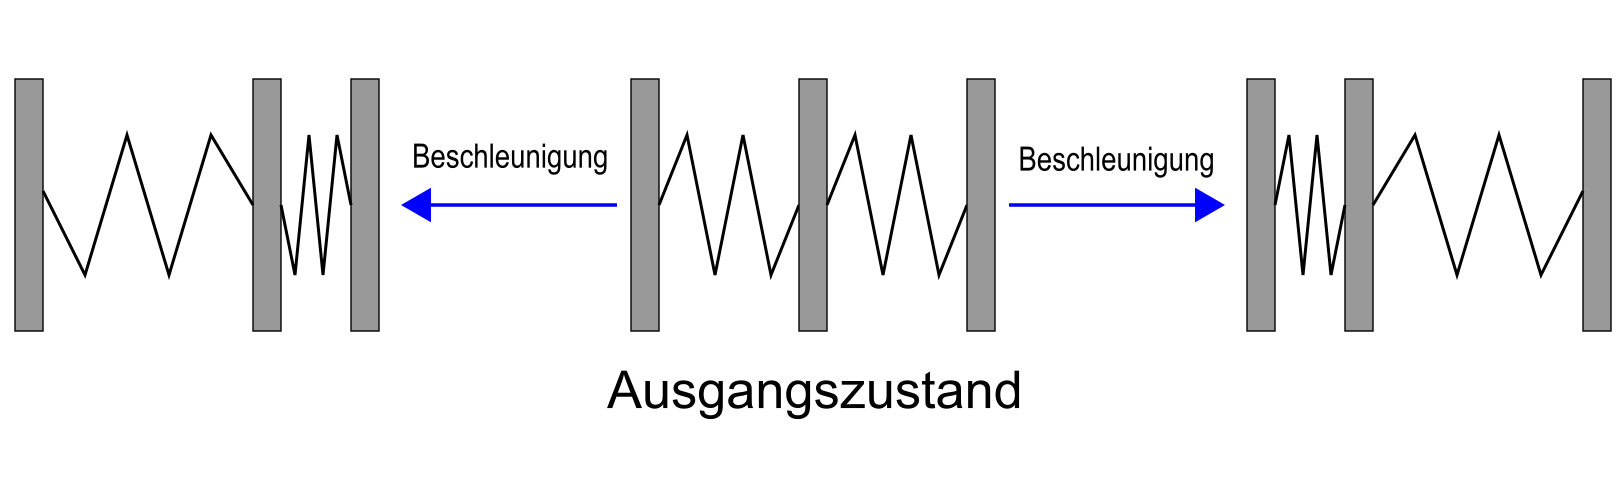
\includegraphics[width=0.7\linewidth]{images/Beschleunigungssensor.png}
	\caption[Beschleunigungssensor]{Beschleunigungssensor}
	\label{fig:Beschleunigungssensor}
\end{figure}

\textbf{Beschleunigungssensor}

Ein Beschleunigungssensor funktioniert nach dem selben Prinzip, wie ein Gyroskop. Der einzige Unterschied ist, dass der Sensor die Beschleunigung in Richtung der x-, y- und z-Achse deklariert. Ein Gyroskop bezieht sich lediglich auf die Bewegung, um die Achsen, also befindet es sich in Ruhestellung, liefert es den Wert Null für alle drei Dimensionen (x,y,z). \textcite{MPU6050} Die Module haben die Achsen aufgedruckt.

\begin{figure}[H]
	\centering
	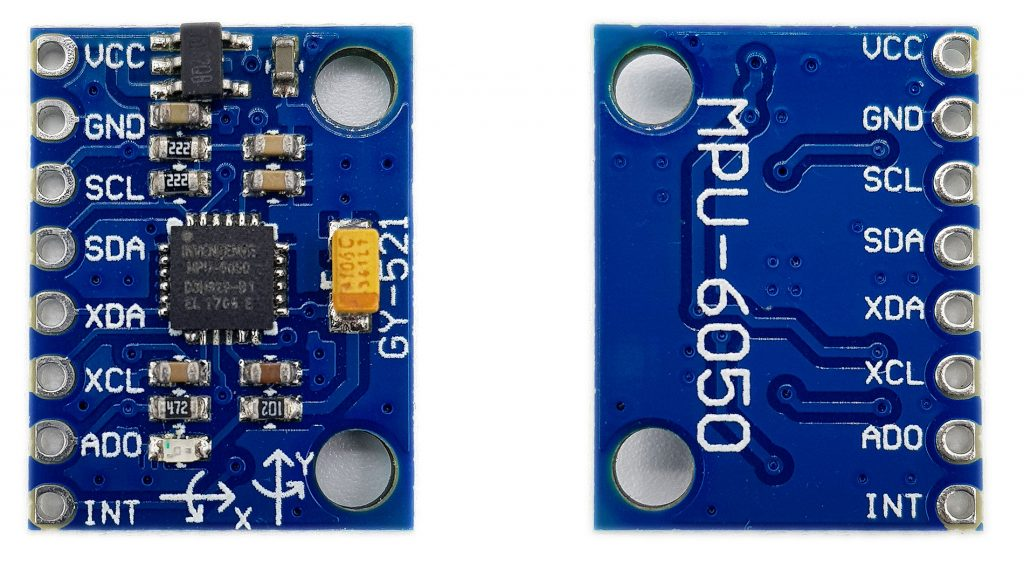
\includegraphics[width=0.7\linewidth]{images/Modul.jpg}
	\caption[Modul]{Modul}
	\label{fig:Modul}
\end{figure}

\subsection{Trägheitsnavigation}

Die Trägheitsnavigation nutzt die physikalische Eigenschaften der Trägheit, um fortlaufende Berechnung der Position, Orientierung und Geschwindigkeit eines Objekts zu ermöglichen. \textcite{Traegheitsnavigation} Es ist immer nur die Anfangsposition bekannt, anhand dieser wird die spätere Position eines Objektes errechnet. Auch in GPS-gestörten Umgebungen z.B. Gebäuden, funktioniert die Trägheitsnavigation. 


\section{Software}


\subsection{Mobil Apps Grundlagen}

\textbf{Native Apps}

Native Apps (\emph{=deu.: angepasste Anwendung}) sind Anwendungen, die speziell für ein Betriebssystem (Android, iOS) entwickelt wurden. \textcite{NativeApps}

\textbf{Android}

Android ist einer der weltweit Bekanntesten Betriebssysteme, es ist akutell auf 2,5 Milliarden aktiven Geräten installiert. \textcite{Android} Weiters ist Android ein Open-Source Betriebssystem, es ist offen für Entwickler.  

\textbf{iOS}

Das Betriebssystem iOS wurde von Apple im Jahre 2007 veröffentlicht. \textcite{iOS} Die Software wird bei iPhone und iPad verwendet. Anders wie bei Android ist iOS nicht quelloffen, außerdem werden keine Betriebssystem-Lizenzen vergeben. Man benötigt eine gültige Apple-ID, um das Gerät zu verwenden.

\subsection{Cross-Platform-Apps}

\textbf{Flutter}

Flutter ist eine Open-Source-Software, welche von Google entwickelt worden ist.\textcite{Flutter} Der Vorteil dieses Frameworks ist, dass man mit einem Programmcode in Flutter mehreren Apps auf verschiedenen Plattformen (Android, iOS) erstellen kann. Die Hauptprogrammiersprache ist Dart.

\textbf{React Native}

React Native ist eine Open-Source-Software, welche von Facebook entwickelt worden ist. \textcite{ReactNative} Es wurde entwickelt, um Entwicklern mit Erfahrungen in React die Möglichkeit zu geben, einfacher Android Apps basierend auf React zu entwicklen. Die Hauptprogrammiersprachen sind JavaScript oder TypeScript.

\subsection{App-Entwicklung}

Für die App-Entwicklung wird Android Studio verwendet. 

Um Android Studio verwenden zu können muss man eine SDK (\emph{=engl. Software Development Kit}) installieren. \textcite{AppEntwicklung} Außerdem ist IntelliJ IDEA Community/Ultimate als IDE (\emph{=engl. Integrated Development Environment}) vorgesehen. Diese enthält die wichtigsten Programmierwerkzeuge und Programmierbiblotheken. Der Entwickler, selbst, entscheidet darüber, welche Programmiersprache verwendet wird. Es besteht die Auswahl zwischen Java, Kotlin, Ruby oder sogar C++.


\textbf{IntelliJ IDEA}

IntelliJ IDEA ist einer der beliebtesten IDEs für Java und Kotlin, die es auf den Markt gibt. Das Unternehmen, welches die Software entwickelt hat, heißt JetBrains. 

Es gibt zwei verschiedene Versionen:
\begin{itemize}
	\item IntelliJ IDEA Community Edition
	\item IntelliJ IDEA Ultimate
\end{itemize}

Die beiden Versionen unterscheiden sich minimal, denn die Ultimate Version bietet z.B. JavaScript Integration oder "duplicate detection". \textcite{IntelliJ}

\begin{figure}[H]
	\centering
	\includegraphics[width=0.5\linewidth]{images/intelliJ.png}
	\caption[IntelliJ]{IntelliJ}
	\label{fig:IntelliJ}
\end{figure}

\textbf{Eclipse}

Eclipse ist eine weitere bekannte IDE, die Software umfasst 48\% des Marktanteils. Man kann nicht nur in Java programmieren, sondern mit den entsprechenden Plugins auch in Python, JavaScript oder C++. Außerdem läuft es auf jeder Platform, Linux, macOS oder Windows, \textcite{Eclipse}.
Eclipse ist eine weitere bekannte IDE, die Software umfasst 48\% des Marktanteils. Man kann nicht nur in Java programmieren, sondern mit den entsprechenden Plugins auch in Python, JavaScript oder C++. Außerdem läuft es auf jeder Platform, Linux, macOS oder Windows.

\begin{figure}[H]
	\centering
	
\includegraphics[width=0.5\linewidth]{images/eclipse.png}
	\caption[Eclipse]{Eclipse}
	\label{fig:Eclipse}
\end{figure}

\section {Vergleich verschiedener Programmiersprachen}
Wie aus der Statistik abzulesen sind Python, Java, JavaScript, C\# und C/C++ die 5 aktuell meistverwendeten Programmiersprachen der Welt. \textcite{meistProgrammiersprachen}


\begin{figure}[H]
	\centering
	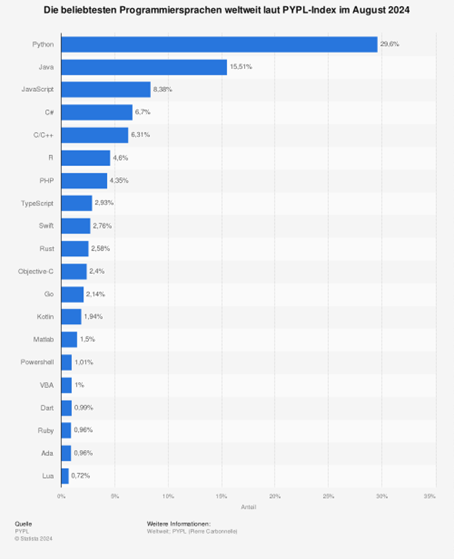
\includegraphics[width=0.7\linewidth]{images/Programmiersprachen.png}
	\caption[Programmiersprachen]{Programmiersprachen}
	\label{fig:Programmiersprachen}
\end{figure}

\subsection{Python}
Bei Python wird der Quellcode zur Laufzeit in Bytecode übersetzt, so zeichnet sich diese Programmiersprache durch eine schnelle Entwicklungszeit aus. Python findet Anwendung in der Webentwicklung, Netzwerkprogrammierung sowie der Datenanalyse. Darüber hinaus wird diese Programmiersprache auch für die Automatisierung von Prozessen eingesetzt. \textcite{Programmiersprachen}


\textbf{Vorteile}
\begin{itemize}
	\item einfache Syntax
	\item kein manuelles Speichermanagement notwendig
	\item plattformunabhängiger Code
	\item stellt eine breite Auswahl an installierbaren Bibliotheken, Frameworks und umfassenden Support bereit
\end{itemize}

\textbf{Nachteile}
\begin{itemize}
	\item höherer Speicherbedarf
	\item für mobile Anwendungen gibt es nur eine begrenzte Unterstützung für die Entwicklungen
	\item langsamere Ausführungsgeschwindigkeit im Vergleich zu anderen Programmiersprachen
\end{itemize}

\subsection{Java}
Die umfangreiche Verbreitung und Beliebtheit von Java hat im Laufe der Zeit zu einer umfassenden Bibliothek geführt, die eine Vielzahl von Klassen und Funktionen für einige Anwendungsbereiche bereitstellt. Dies ermöglicht Entwicklern für häufig benötigte Lösungen auf bestehende Ressourcen zurückzugreifen und diese zu integrieren. \textcite{Programmiersprachen}

\textbf{Vorteile}
\begin{itemize}
	\item plattformunabhängigkeit durch die Ausführung über einer virtuellen Java-Maschine
	\item objektorientierte Programmierung, die eine klare Strukturierung und eine effektive Wiederverwendung von bestehendem Code ermöglicht
	\item Fehlererkennung und integrierte Sicherheitsmaßnahmen sorgen für hohe Sicherheit und Robustheit
	\item kein manuelles Speichermanagement erforderlich
	\item Skalierbarkeit unterstützt die Entwicklung großer und komplexer Anwendungen
\end{itemize}

\textbf{Nachteile}
\begin{itemize}
	\item längere Entwicklungs- und Einarbeitungszeiten aufgrund komplexer Strukturen und einer strikteren Syntax
	\item erhöhter Speicherbedarf
	\item mögliche Lizenzgebühren für die kommerzielle Nutzung
	\item fehlende Unterstützung bei Echtzeitanwendungen
\end{itemize}

\subsection{JavaScript}
JavaScript war ursprünglich eventbasiert - das heißt, der JavaScript - Code war so strukturiert, dass er auf Benutzerinteraktionen und Ereignisse reagiert, anstatt selbst aktiv zu werden. Diese Programmiersprache kommt heutzutage auch auf Servern und in Mikrocontrollern nicht nur in Webbrowsern zum Einsatz. \textcite{Programmiersprachen}

\textbf{Vorteile}
\begin{itemize}
	\item große Unterstützung von allen bekannten Webbrowsern
	\item plattformunabhängige Ausführung des Codes im Browser
	\item breite Community und eine weite Verbreitung
	\item leichte Erstellung interaktiver Webseiten und kleinerer Anwendungen
\end{itemize}

\textbf{Nachteile}
\begin{itemize}
	\item browserabhängige Interpretation des Codes ermöglicht es, dass es zu Abweichungen kommen kann und soll bei der Entwicklung beachtet werden
	\item geringere Performance im Vergleich zu anderen Programmiersprachen
	\item geringe Skalierbarkeit
\end{itemize}

\subsection{C\#}
C\# ist eine stark typisierte Programmiersprache, sie erfordert zwar einen größeren Aufwand, bietet aber eine verbesserte Fehlererkennung, was zu einer geringeren Anzahl an Bugs führt. Diese Programmiersprache ist speziell für die Entwicklung von Desktop-, Cloud-, Webanwendung, Spiele und mobilen Apps im Microsoft Umfeld ausgelegt. \textcite{Programmiersprachen}

\textbf{Vorteile}
\begin{itemize}
	\item dauerhafte Weiterentwicklung mit neuen Features
	\item große Community, die viele Tools und Unterstützungen anbieten
	\item integration in die Microsoft Umgebung und dessen verbundenen Ressourcen
	\item breites .NET-Framework mit großer Bibliothek und einigen Tools, sowie Funktionen
\end{itemize}

\textbf{Nachteile}
\begin{itemize}
	\item viele Konzepte und Funktionen, die aufwendig zum Erlernen sind
	\item eingeschränkte Plattformunabhängigkeit, deshalb eignet sich diese Programmiersprache hauptsächlich für Windows-Anwendungen
\end{itemize}

\subsection{C/C++}
Die Programmiersprache C ist eine der wenigen, die sich zum Programmieren von Betriebssystemen eignet. Weiters ist C bis heute der Standard für Betriebssysteme, Treiber und Embedded Systeme. C++ kombiniert die Vorteile der Kontrolle über die Hardware mit den Konzepten der objektorientierten Programmierung. Wird in Bereichen wie Spieleentwicklung über die Grafikprogrammierung bis hin zu Echtzeit Systemen zum Einsatz gebracht. \textcite{Programmiersprachen}

\textbf{Vorteile}
\begin{itemize}
	\item schnell und effizient durch die direkte Ausführung auf der CPU
	\item Hardware nahes Programmieren und der direkte Zugriff auf den Speicher ermöglichen manuelle Optimierungen
	\item großes Anwendungsgebiet und vielseitige Einsatzmöglichkeiten
	\item bietet durch C++ eine prozedurale als auch eine objektorientierte Programmierung
	\item sehr gute Skalierbarkeit
\end{itemize}

\textbf{Nachteile}
\begin{itemize}
	\item fehleranfällig aufgrund direkter Speicherkontrolle und -verwaltung
	\item schlechte Code könnte Sicherheitslücken eröffnen, wo sich Hacker Zugriff schaffen können
\end{itemize}



\subsection{Kotlin}
Kotlin wird für die Entwicklung von Android-Apps verwendet. Außerdem bietet diese Programmiersprache eine saubere und präzise Syntax im Vergleich zu Java. Zudem kann ein bestehender Java-Code problemlos in Kotlin Projekte integriert werden, dass selbe funktioniert auch umgekehrt. \textcite{Kotlin}

\textbf{Vorteile}
\begin{itemize}
	\item Sicherheit: durch die Unterstützung von immutablen Daten führt es zu wenigen Fehlern im Code
	\item Kotlin kann problemlos mit Java-Code und Bibliotheken zusammenarbeiten
	\item bietet eine moderne Syntax, die die Lesbarkeit und Wartbarkeit verbessert
\end{itemize}

\textbf{Nachteile}
\begin{itemize}
	\item weniger erfahrene Kotlin Entwickler als bei Java
	\item geringere Communitygröße
\end{itemize}


\section{Entwicklungsumgebungen}
Eine integrierte Entwicklungsumgebung ist eine Softwareanwendung, die alle Werkzeuge, die für ein Softwareentwicklungsprojekt benötigt werden, an einem Ort vereint. Einige IDEs sind auf eine spezifische Programmiersprache wie Python oder Java ausgerichtet. Die Mehrheit der IDEs ist jedoch so konzipiert, dass sie mit einer Vielzahl unterschiedlicher Programmiersprachen kompatibel ist. Die bekanntesten Anbieter von integrierten Entwicklungsumgebungen sind Visual Studio, IntelliJ IDEA, Microsoft, JetBrains. 

\subsection{Funktionen von IDEs}
Alle integrierten Entwicklungsumgebungen beinhalten einen Texteditor, der die Erstellung und Bearbeitung von Quellcode ermöglicht. Darüber hinaus bieten einige IDEs visuelle Komponenten und Drag-and-Drop-Schnittstellen für die Entwicklung von Frontend-Komponenten an. Üblicherweise sind diese Editoren mit einer Syntaxhervorhebung ausgestattet, um die Lesbarkeit und Fehlererkennung im Code zu erleichtern. Debugging-Tools unterstützen Anwender bei der Behebung von Fehlern im Quellcode. Profiling ermöglicht die Analyse von Laufzeit, CPU-Auslastung von Programmen und Speicherverbrauch, um Leistungsengpässe sowie Optimierungspotenziale durch eine Visualisierung von Daten zu identifizieren. 

\subsection{Arten von IDEs}
\textbf{Mehrsprachige integrierte Entwicklungsumgebungen} sind mit einer Vielzahl von Programmiersprachen kompatibel. Zu den bekanntesten gehört Visual Studio, das für seine umfangreichen Funktionen und regelmäßigen Updates geschätzt wird. Die Unterstützung für zusätzliche Programmiersprachen kann durch die Installation von Erweiterungen integriert werden. Mit dem Aufkommen der mobilen App-Entwicklung haben sich spezialisierte IDEs für diesen Bereich etabliert. Diese Plattformen ermöglichen Entwicklern die Erstellung effizienter und umfassender mobiler Anwendungen. Beispiele hierfür sind Android Studio für die Android-Entwicklung und Xcode für die iOS-Entwicklung.

Gegenüber lokalen Entwicklungsumgebungen bieten \textbf{Web- oder Cloud basierte IDEs} mehrere Vorteile. Eine SaaS-IDE (Software as a Service) ermöglicht es, Aufgaben auszuführen, ohne die Ressourcen einer lokalen Workstation zu belasten. Diese cloudbasierten IDEs sind oft plattformunabhängig und können nahtlos mit verschiedenen Cloud-Anbietern integriert werden.
Sprachspezifische IDEs hingegen richten sich an Entwickler, die ausschließlich mit einer einzigen Programmiersprache arbeiten möchten. Beispiele hierfür sind Jikes und Jcreator für Java, CodeLite und C-Free für C/C++, sowie Idle für Python. \textcite{integrierteEntwicklungsumgebung}



\section{Vergleich Single Board Computer und Mikrocontrollern}
\subsection{Single Board Computer}
Einplatinencomputer (Single-Board Computers, SBCs) sind Computersysteme, bei denen sämtliche notwendigen Komponenten, wie Prozessor, Speicher und Ein-/Ausgabeschnittstellen, auf einer einzigen Platine integriert sind. Diese Geräte fungieren oft als Hauptprozessor in eingebetteten Systemen oder werden als kostengünstige Allzweckcomputer eingesetzt.

\textbf{Vorteile}
\begin{itemize}
	\item kompakte Bauweise
	\item geringes Gewicht
	\item flexible Einsatzmöglichkeit
	\item reduzierten Energieverbrauch 
	\item niedrige Kosten
	\item benutzerfreundlich
	\item erfordern minimale Vorbereitungen für den Betrieb
\end{itemize}

\textbf{Nachteile}
\begin{itemize}
	\item hohe Kosten, da sie viele Funktionen und Komponenten beinhalten
	\item größer und schwerer als Mikrocontroller
	\item hoher Stromverbrauch
\end{itemize}

\subsubsection{Arten von SBCs}
Einplatinencomputer lassen sich in drei Hauptkategorien unterteilen: einem Mikrocontroller basierten, einem Mikroprozessor basierten und einem FPGA basierten System. 

Die einfachste und kostengünstigste Art ist ein \textbf{Mikrocontroller basierter Einplatinencomputer}. Mikrocontroller-basierte SBCs zeichnen sich in der Regel durch einen einzigen Mikrocontroller-Chips aus, der alle grundlegenden Funktionen des Systems übernimmt, einschließlich Ein- und Ausgabe, Speicher und Energieverwaltung. 

Im Gegensatz dazu verfügen \textbf{mikroprozessorbasierte SBCs} über einen Mikroprozessor anstelle eines Mikrocontrollers, was eine höhere Leistungsfähigkeit verleiht. Mikroprozessoren sind vielfältiger und in der Lage, anspruchsvollere Aufgaben zu bewältigen. 

Die leistungsstärkste Kategorie von SBCs sind \textbf{FPGA-basierte Systeme}, die mit einem Field-Programmable Gate Array (FPGA) ausgestattet sind. FPGAs sind vielseitige Chips, die so programmiert werden können, dass sie verschiedene Arten von Logikchips nachbilden, einschließlich Mikroprozessoren oder Mikrocontrollern, und damit eine hohe Flexibilität und Leistungsfähigkeit bieten.

\subsubsection{Typen von SBCs}
Es existieren verschiedene Typen von Einplatinencomputern. Der Raspberry Pi ist ein weit verbreiteter, kostengünstiger Singleboard Computer. Weitere leistungsstärkere Modelle umfassen den BeagleBone und die Odroid-Serie, die ebenfalls breite Anwendung finden.

\subsubsection{Betriebssysteme für SBCs}
Die meisten SBCs laufen mit Linux-basierten Betriebssystemen wie Raspbian, Ubuntu oder Fedora. Daneben können auch andere Betriebssysteme wie Windows 10 IoT Core und Android auf SBCs verwendet werden. \textcite{EinplatinencomputerSBCs}

\begin{figure}[H]
	\centering
	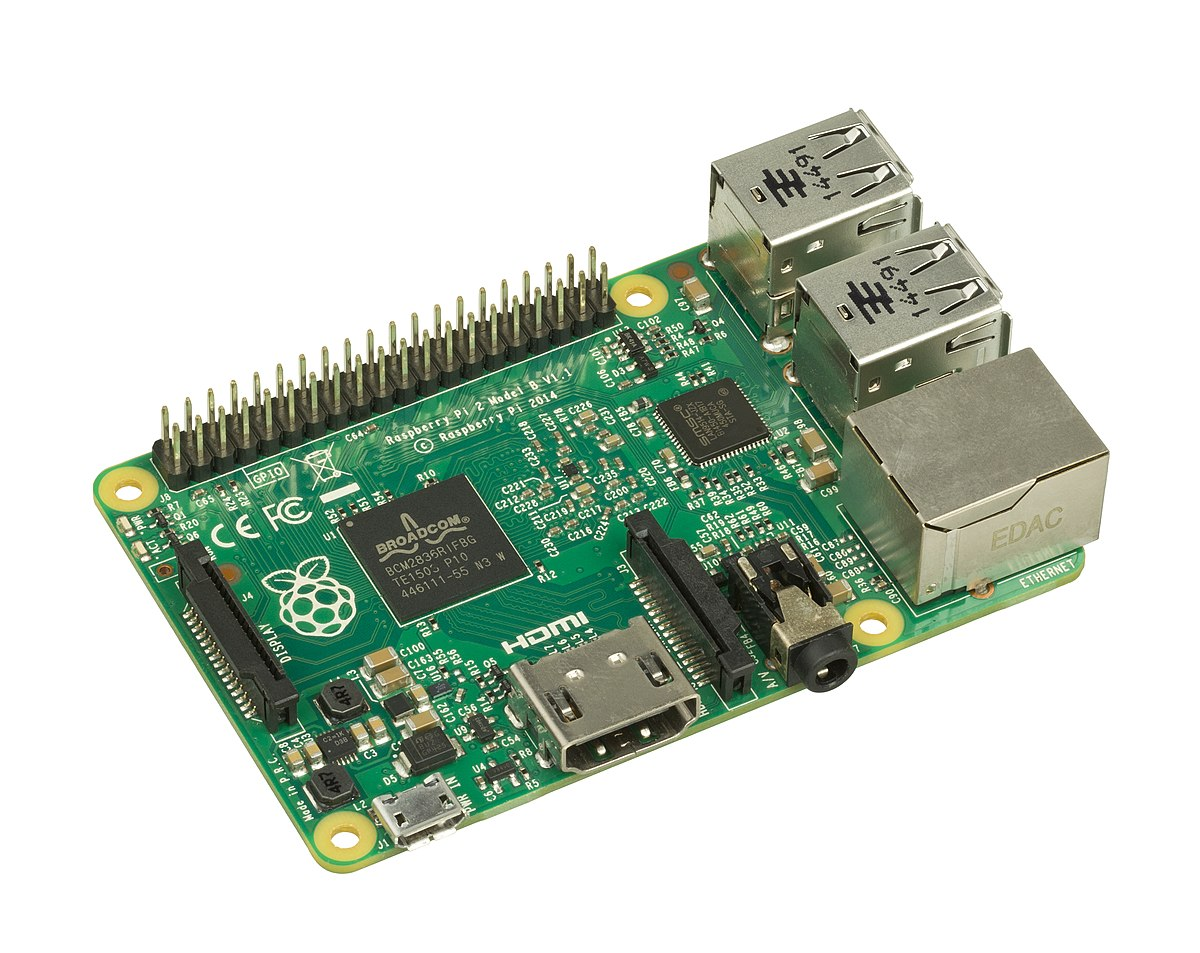
\includegraphics[width=0.7\linewidth]{images/SingleBoard Computer.jpg}
	\caption[SingleBoard Computer]{SingleBoard Computer}
	\label{fig:Single Board Computer}
\end{figure}

\subsection{Mikrocontroller}
Sind kleine Computer-Systeme, die für eine begrenzte Anzahl von Aufgaben entwickelt wurden. Mikrocontroller enthalten einen Prozessor, Speicher und I/O-Ports. Häufig werden sie für einfachere Anwendungen wie die Steuerung von Geräten und Maschinen verwendet. \textcite{EinzelplatinencomputerVsMikrocontroller}

\textbf{Vorteile}
\begin{itemize}
	\item kosteneffizienter als SBCs
	\item geringer Stromverbrauch
	\item klein und leicht, geeignet für Projekte wo man tragbare Geräte benötigt 
\end{itemize}

\textbf{Nachteile}
\begin{itemize}
	\item keine Netzwerkfähigkeiten oder Anschlüsse für externe Geräte
	\item beschränkte Funktionalitäten, komplexere Aufgaben können teilweise nicht ausgeführt werden
\end{itemize}

\begin{figure}[H]
	\centering
	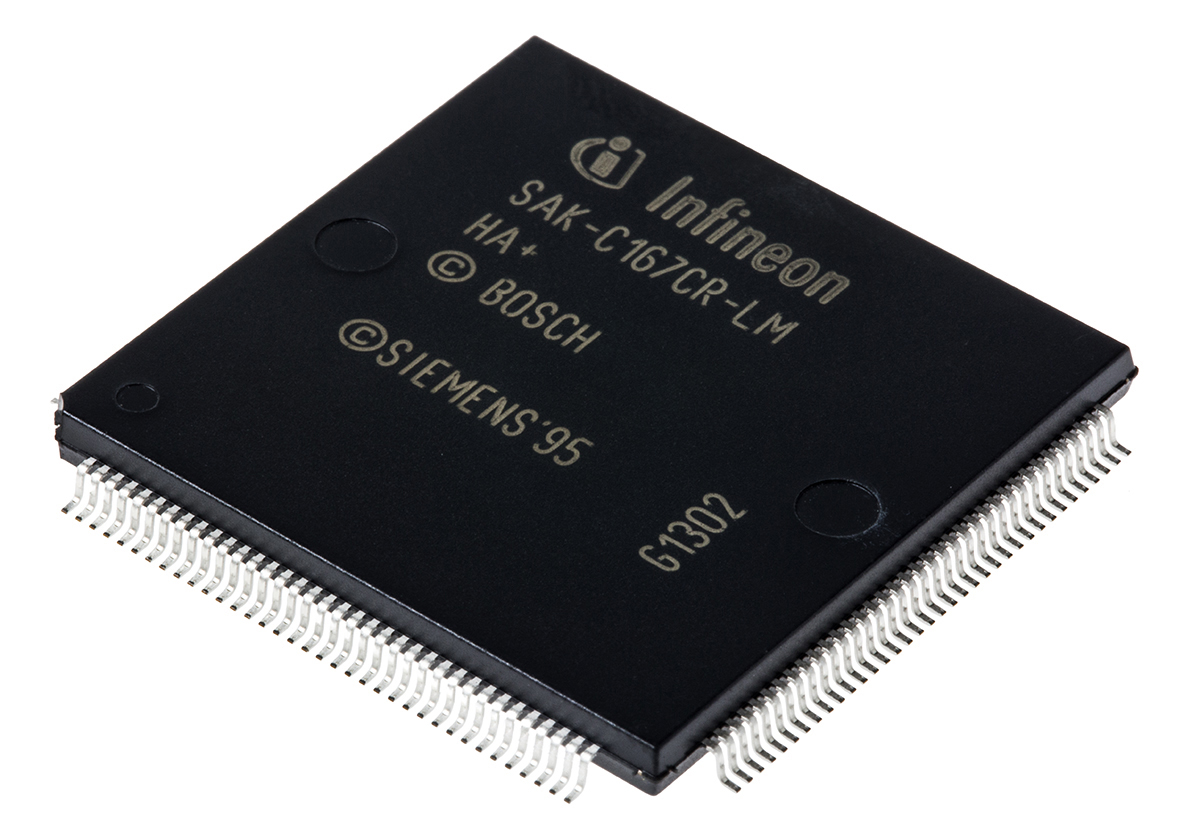
\includegraphics[width=0.7\linewidth]{images/Mikrocontroller.jpg}
	\caption[Mikrocontroller]{Mikrocontroller}
	\label{fig:Mikrocontroller}
\end{figure}


\section{Vergleich verschiedener Betriebssysteme}
\subsection{Windows}
Windows ist mit fast jedem Programm, das auf den Markt kommt, kompatibel. Das Betriebssystem ist einfach und auch für Nutzer ohne Kenntnisse verständlich aufgebaut. Aufgrund der vielen Windows-kompatiblen Programme ist dieses Betriebssystem für professionelle Anwendungen sowie für Unterhaltungszwecke gedacht. Dank der aktiven Community von Windows werden zahlreiche Hilfsangebote bereitgestellt.

\textbf{Vorteile}
\begin{itemize}
	\item auf den meisten Geräten vorinstalliert
	\item breites Angebot an Software
	\item für Einsteiger gut geeignet
\end{itemize}

\textbf{Nachteile}
\begin{itemize}
	\item komplexes System
	\item Lizenzgebühren
	\item häufig das Ziel von Malware
	\item wird mit zunehmender Nutzungsdauer langsamer
\end{itemize}

\subsection{Linux}
Linux wird häufig von Menschen, die sich professionell mit IT beschäftigen genutzt, da die meisten Linux-Distributionen hohe Einstiegsbürden haben. Zudem besteht die Möglichkeit, dass Windows-Programme auch unter Linux laufen. Durch die breite Community findet man in Onlineforen und auf verschiedenen Webseiten zu jedem Problem Hilfe. \textcite{LinuxVsWindows}

\textbf{Vorteile}
\begin{itemize}
	\item meisten Linux-Distributionen sind kostenlos
	\item Linux-Kernel und Distributionen sind quelloffen
	\item umfangreich konfigurierbar
	\item selten Ziel von Viren und Malware
	\item schnelle Laufzeit
\end{itemize}

\textbf{Nachteile}
\begin{itemize}
	\item begrenzte Auswahl an Software
	\item für Einsteiger schwieriger
\end{itemize}

\subsubsection{Distributionen}
Linux-Distributionen bieten eine große Anzahl an Programmen, die in den Repositories zur Installation bereitstehen. Häufig genutzte Linux-Distributionen sind Debian, Red Hat und Ubuntu, doch es gibt noch viel mehr Distributionen, die in der Open-Source-Variante oder fortlaufend weiterentwickelt werden.\textcite{LinuxDistribution}

\subsubsection{Debian}
Eines der beliebtesten Systeme auf Basis des Linux-Kernels ist Debian Linux-OS. Es ist eines der ältesten und stabilsten Linux Distributionen. Debian wird gerne für den Betrieb von Servern verwendet. Weiters dient Debian als Software-Grundlage für Ubuntu, das mit Abstand beliebteste Linux-Betriebssystem. \textcite{DebianLinuxOS}

\textbf{Vorteile}
\begin{itemize}
	\item gute Stabilität
	\item einige Software Optionen
	\item große Community
	\item wenige Anforderungen an die Hardware
\end{itemize}

\textbf{Nachteile}
\begin{itemize}
	\item komplizierte Installation und Nutzung
	\item unregelmäßige Updates
	\item teils veraltete Software
	\item viele Softwareanwendungen werden nicht unterstützt
\end{itemize}


\subsubsection{Ubuntu}
Ubuntu hat einige Derivate wie Kubuntu, Xubuntu, Lubuntu und viele mehr. Diese unterscheiden sich jeweils mit einer anderen Desktop Oberfläche. Der Ubuntu Desktop bietet ein modernes, kostenloses, einfach zu bedienendes und stabiles Betriebssystem. \textcite{UbuntuVsDebian} \textcite{WarumUbuntu}

\textbf{Vorteile}
\begin{itemize}
	\item benutzerfreundlich
	\item einfache Installation und Nutzung
	\item breite Auswahl an Software
	\item hohe Anpassungsfähigkeit
\end{itemize}

\textbf{Nachteile}
\begin{itemize}
	\item manchmal bereitet Ubuntu Probleme nach Updates
	\item größere Ansprüche an die Hardware
\end{itemize}


\subsubsection{Red Hat}
Red Hat ist die älteste LTS (Long Term Support) Distribution. Im Vergleich zu Ubuntu und Debian hat Red Hat ein eingeschränktes Paketangebot, es wird nur die Desktopumgebung GNOME unterstützt. Komponenten wie der Kernel bleiben auf einer Version und werden im Laufe der Zeit stark angepasst. Weshalb auch neuere Hardware mit älteren Distributionen funktionsfähig sind. \textcite{RedHatEnterpriseLinux}

\textbf{Vorteile}
\begin{itemize}
	\item lange Support Dauer
	\item regelmäßige Minor-Releases, die sich an aktuelle Hardware anpassen
\end{itemize}

\textbf{Nachteile}
\begin{itemize}
	\item beschränktes Softwareangebot 
	\item keine Distributionsupgrades zwischen Hauptversionen möglich
	\item mit jedem Minor-Release werden Programmversionen angehoben, weshalb die Softwareversionen nicht wirklich stabil ist
\end{itemize}


\section{Virtuelle Maschine}
Eine Virtuelle Maschine ist ein virtueller Rechner, der den Endnutzern einen physischen Rechner sowie eine Hardware und ein Betriebssystem bereitstellt. VMs ermöglichen die gleichzeitige Ausführung von unterschiedlichen Betriebssystemen auf verschiedenen virtuellen Computern. Dadurch kann das Betriebssystem Linux auf einem Windows Betriebssystem laufen oder ältere Windows Versionen auf einem neuen Windows Betriebssystem laufen. \textcite{WasIstEineVirtualMachine}
\textcite{VirtuelleMaschineDefinition} \textcite{VirtualMachineAdvantagesAndDisadvantages}

\textbf{Vorteile}
\begin{itemize}
	\item schnell und einfache Installation eines Betriebssystems auf einem physischen Server
	\item hohe Sicherheit, da sich Malware oder Angriffe nicht über mehrere Maschinen ausbreiten können
	\item benötigen weniger Hardwareressourcen 
	\item flexibel, da mehr als eine virtuelle Maschine erstellt werden kann
	\item schnelle Wiederherstellung, falls Daten verloren gehen oder ein Systemabsturz ist
\end{itemize}

\textbf{Nachteile}
\begin{itemize}
	\item langsamer als reale Maschinen
	\item schwierig zu konfigurieren, wenn man sich nicht auskennt, dies kann in einer Firma zu sehr hohen Kosten kommen
	\item zu wenig Speicherplatz für Virtuelle Maschinen am Computer oder Laptop kann sehr teuer werden
\end{itemize}


\section{Virtualisierung}
Virtualisierung ermöglicht physische Hardware-Ressourcen in virtuelle Maschinen aufzuteilen, wodurch mehrere virtuelle Instanzen auf einem physischen Server ausgeführt werden können.

\subsection{Arten der Virtualisierung}
\subsubsection{Hardware-Virtualisierung}
Bei einer Hardware-Virtualisierung werden Hardware-Komponenten mittels Software bereitgestellt. Ein Beispiel zu einer Virtualisierung von einer Hardware wäre eine Virtuelle Maschine. Die Abstraktionsschicht erzeugt zwischen der physischen Grundlage und dem virtuellen System verschiedene Typen von Hypervisoren. Ein Hypervisor ist eine Software, die den Betrieb mehrerer Gastsysteme auf einem Wirtsystem ermöglicht.

\textbf{Vollvirtualisierung:} Hier spielt der Hypervisor jeder VM eine Hardware Umgebung vor. Jede Virtuelle Maschine hat dadurch einen zugewiesenen Anteil an virtuellen Hardware-Ressourcen und kann auf dieser Grundlage Anwendungen ausführen. Beliebte Software-Lösungen sind Oracle VM VirtualBox, Parallels Workstation und VMware Workstation.

\textbf{Paravirtualisierung:} Hier stellt der Hypervisor nur eine Programmierschnittstelle (API) zur Verfügung, wo die Gastsysteme auf die physische Hardware des Wirtssystems zugreifen kann. Der Kernel des Gastsystems muss für die API portiert werden. Somit lassen sich nur modifizierte Gastbetriebssysteme paravirtualisieren. 

\subsubsection{Desktop-Virtualisierung}
Bei einer Hardware-Virtualisierung werden Hardware-Komponenten mittels Software bereitgestellt. Ein Beispiel zu einer Virtualisierung von einer Hardware wäre eine Virtuelle Maschine. Die Abstraktionsschicht erzeugt zwischen der physischen Grundlage und dem virtuellen System verschiedene Typen von Hypervisoren. Ein Hypervisor ist eine Software, die den Betrieb mehrerer Gastsysteme auf einem Wirtsystem ermöglicht.

\textbf{Vollvirtualisierung:} Hier spielt der Hypervisor jeder VM eine Hardware-Umgebung vor. Jede Virtuelle Maschine hat dadurch einen zugewiesenen Anteil an virtuellen Hardware-Ressourcen und kann auf dieser Grundlage Anwendungen ausführen. Beliebte Software-Lösungen sind Oracle VM VirtualBox, Parallels Workstation und VMware Workstation.

\textbf{Paravirtualisierung:} Hier stellt der Hypervisor nur eine Programmierschnittstelle (API) zur Verfügung, wo die Gastsysteme auf die physische Hardware des Wirtssystems zugreifen kann. Der Kernel des Gastsystems muss für die API portiert werden. Somit lassen sich nur modifizierte Gastbetriebssysteme paravirtualisieren. \textcite{WasIstVirtualisierung}

\subsection{Programme}
\subsubsection{VMware}
VMware ermöglicht die Virtualisierung der x86-Betriebssysteme auf einem normalen Desktop-PC. Wie bei den meisten VM-Programmen lassen sich sogenannte Snapshots der virtuellen Maschine machen, um dies zu einem späteren Zeitpunkt wiederherzustellen. Zudem lässt VMware einen zusätzlichen Desktop betreiben, welcher besonders abgesichert ist. Kostenmäßig ist die VMware bei circa 200\texteuro{}. Eine Testversion lässt sich 30 Tage lang nutzen und Personen, die eine Hochschule oder Universität besuchen gibt es einen Rabatt. 

\begin{figure}[H]
	\centering
	
\includegraphics[width=0.3\linewidth]{images/VMware.png}
	\caption[VMware]{VMware}
	\label{fig:VMware}
\end{figure}


\subsubsection{Oracle VM VirtualBox}
Die VirtualBox gilt als „Free-and-Open-Source-Software”, was bedeutet, dass die Software unter einer Lizenz erhältlich ist, somit ist es kostenlos zu verwenden, zu verändern und zu verteilen. Diese Virtuelle Maschine ist eine Grundlage für den Betrieb von virtuellen Maschinen auf einem Host-System und wird oft in spezialisierter Software eingesetzt. Das Tool „Vagrant“ automatisiert die Erstellung reproduzierbarer Entwicklungsumgebungen. Dabei dient Vagrant als Schnittstelle zwischen Virtualisierungssoftware wie VirtualBox, VMware, Hyper-V und Docker. Diese VM lässt sich kostenlos nutzen. 

\begin{figure}[H]
	\centering
	
\includegraphics[width=0.5\linewidth]{images/VirtualBox.jpg}
	\caption[VirtualBox]{VirtualBox}
	\label{fig:VirtualBox}
\end{figure}

\subsubsection{Parallels}
Nutzer können bei dieser VM am Mac mit mehreren Betriebssystemen arbeiten. Hier liegt der Fokus auf dem Bereitstellen einer Windows Desktop Umgebung die parallel zu macOS läuft. Parallels ermöglicht nahtlose Verschiebungen und Freigeben von Inhalten zwischen Mac und Windows. Diese VM-Lizenz kostet circa 100\texteuro{}. Privatnutzer und Schüler bekommen einen Rabatt. \textcite{VirtualisierungsSoftware}

\begin{figure}[H]
	\centering
	
\includegraphics[width=0.5\linewidth]{images/Parallels.jpg}
	\caption[Parallels]{Parallels}
	\label{fig:Parallels}
\end{figure}

\section{Vergleich von GitHub und GitLab}
\subsection{GitHub}
GitHub ist eine Cloud-basierte Plattform, auf der Code gespeichert, sowie geteilt wird und man mit anderen Personen zusammenarbeiten kann. Dateien werden in GitHub hochgeladen und in einem Repository gespeichert. Bei Änderungen der Dateien wird GitHub automatisch beginnen die Änderungen nachzuverfolgen und zu verwalten. Sobald mehrere Personen an einem Repository zusammenarbeiten, müssen die Änderungen von allen Mitarbeitern auf GitHub abgerufen, sowie die eigenen Änderungen an das Repository auf GitHub gepusht werden. \textcite{GitHubUndGit}

\textbf{Vorteile}
\begin{itemize}
	\item die Arbeit leicht präsentieren oder teilen
	\item Änderungen des Codes jederzeit nachverfolgen, sowie verwalten
	\item an einem Projekt zusammenarbeiten ohne, dass sich die Änderungen auf die Arbeit der Mitarbeiter auswirkt
	\item kostenloser Service
	\item große Community
\end{itemize}

\textbf{Nachteile}
\begin{itemize}
	\item Speicherplatzbeschränkungen, da 100MB in einer Datei nicht überschritten werden können
	\item Repositories sind in der kostenlosen Version auf 1GB beschränkt
\end{itemize}


  \begin{figure}[H]
	\centering
	\includegraphics[width=0.5\linewidth]{images/GitHub.png}
	\caption[GitHub]{GitHub}
	\label{fig:GitHub}
\end{figure}

\section{GitLab}
GitLab ist eine Alternative zu GitHub und wurde entwickelt, um Open Source Projekte zu hosten. Hosting für Wikis und Burg-Tracking Systeme werden angeboten und Berechtigungen für verschiedene Mitarbeiter können entsprechend ihrer Rolle festgelegt als auch geändert werden. Weiters kann man bei GitLab die eigenen Repos kostenlos hosten. GitLab bietet einige sehr interessante Funktionen und ist mittlerweile sehr beliebt geworden.   \textcite{GitHubVsGitLab}

 \textbf{Vorteile}
  \begin{itemize}
  	\item ist eine Open Source Lizenz
  	\item gut in Git integriert
  	\item ermöglicht Self Hosting
  \end{itemize}
  
  \textbf{Nachteile}
  \begin{itemize}
  	\item Benutzeroberfläche ist langsamer als bei GitHub
  	\item häufig Probleme bei Repositories 
  \end{itemize}
  
  
  \begin{figure}[H]
  	\centering
  	
\includegraphics[width=0.5\linewidth]{images/GitLab.png}
  	\caption[GitLab]{GitLab}
  	\label{fig:GitLab}
  \end{figure}
  


\chapter{Ergebnisdokumentation}
\textbf{TBD}



	
	\newpage
	\phantomsection
	\printbibliography[heading=bibintoc]
	
	\listoffigures
	\listoftables
	
	
\chapter*{Begleitprotokoll gem. § 9 Abs. 2 PrO-BHS}\addcontentsline{toc}{chapter}{Begleitprotokoll gem. § 9 Abs. 2 PrO-BHS}


An dieser Stelle wird das Begleitprotokoll eingefügt.
Aus dem Begleitprotokoll soll ersichtlich sein, wer, woran, wann und wie lange, gearbeitet hat.
	
\chapter*{Anhang}\addcontentsline{toc}{chapter}{Anhang}


\begin{itemize}
 \item Projektdokumentation (Kostendarstellung, Besprechungsprotokolle, etc.)
 \item Technische Dokumentation (technische Beschreibungen, Berechnungen, Konstruktionszeichnungen, Versuchsberichte, betriebswirtschaftliche Kalkulationen etc.)
\end{itemize}

Bei der Zusammenstellung der schriftlichen Ausfertigung der Diplomarbeit ist darauf zu achten, dass einerseits die von den Kandidaten / Kandidatinnen jeweils bearbeiteten Teile
diesen eindeutig zugeordnet werden können und andererseits deren Einbindung in das Gesamtprojekt klar zum Ausdruck kommt.

	
	
\end{document}





